\documentclass[8pt,a4paper,compress]{beamer}

\usepackage{/home/siyer/lib/slides}

\title{Lexical Analysis}
\date{}

\begin{document}
\begin{frame}
\vfill
\titlepage
\end{frame}

\begin{frame}
\frametitle{Outline}
\tableofcontents
\end{frame}

\section{Scanning Tokens}
\begin{frame}[fragile]
\pause

The first step in compiling a program is to break it into tokens (aka lexemes); for example, given the \jmm program

\begin{lstlisting}[language=Java]
package pass;

import java.lang.System;

public class Factorial {
    // Two methods and a field
    public static int factorial(int n) {
        if (n <= 0)
            return 1;
        else
            return n * factorial(n - 1);
    }
    
    public static void main(String[] args) {
        int x = n;
        System.out.println(x + "! = " + factorial(x));
    }

    static int n = 5;
}
\end{lstlisting}

we want to produce the sequence of tokens \lstinline{package}, \lstinline{pass}, \lstinline{;},\lstinline{import}, \lstinline{java}, \lstinline{.}, \lstinline{lang}, \lstinline{.}, \lstinline{System},\lstinline{;}, \lstinline{public},\lstinline{class}, \lstinline{Factorial}, \lstinline${$,\lstinline{public}, \lstinline{static}, \lstinline{int},\lstinline{factorial}, \lstinline{(},\lstinline{int}, \lstinline{n,)}, \lstinline${$, \lstinline{if}, \lstinline{(}, \lstinline{n},\lstinline{<=}, \lstinline{0}, \lstinline{)}, \lstinline$}$, \lstinline{return}, \lstinline{1},\lstinline{;}, \lstinline{else},\lstinline{return}, \lstinline{n}, \lstinline{*}, \lstinline{factorial}, \lstinline{(}, \lstinline{n}, \lstinline{-}, \lstinline{1}, \lstinline{)}, \lstinline$}$, \lstinline{;}, \lstinline$}$, \lstinline{public}, \lstinline{static}, \lstinline{void}, \lstinline{main}, \lstinline{(}, \lstinline{String}, \lstinline{[}, \lstinline{]}, \lstinline{args}, \lstinline{)}, \lstinline$}$, \lstinline${$, \lstinline{int}, \lstinline{x}, \lstinline{=}, \lstinline{n}, \lstinline{;}, \lstinline{System}, \lstinline{.}, \lstinline{out}, \lstinline{.}, \lstinline{println}, \lstinline{(}, \lstinline{x}, \lstinline{+}, \lstinline{"!="}, \lstinline{+}, \lstinline{factorial}, \lstinline{(}, \lstinline{x}, \lstinline{)}, \lstinline{)}, \lstinline$}$, \lstinline{;}, \lstinline$}$, \lstinline{static}, \lstinline{int}, \lstinline{n}, \lstinline{=}, \lstinline{5},\lstinline{;}, and \lstinline$}$

\end{frame}

\begin{frame}[fragile]
\pause

We separate the lexemes into categories; in our example program
\begin{itemize}
\item \lstinline{public}, \lstinline{class}, \lstinline{static}, and \lstinline{void} are reserved words

\item \lstinline{Factorial}, \lstinline{main}, \lstinline{String}, \lstinline{args}, \lstinline{System}, \lstinline{out}, and \lstinline{println} are all identifiers

\item The string \lstinline{!=} is a literal, a string literal in this instance

\item The rest are operators and separators
\end{itemize}

\pause
\bigskip

The program that breaks the input stream of characters into tokens is called a lexical analyzer or a scanner

\pause
\bigskip

A scanner may be hand-crafted or it may be generated automatically from a specification consisting of a sequence of regular expressions

\pause
\bigskip

A state transition diagram is a natural way of describing a scanner
\end{frame}

\begin{frame}[fragile]
\pause

A state transition diagram for identifiers and integers and the corresponding code
\begin{center}
\visible<2->{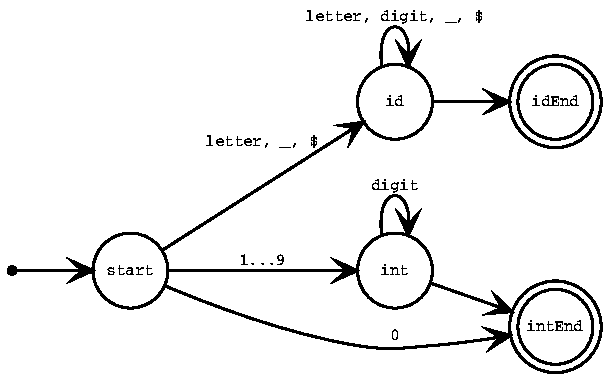
\includegraphics[scale=0.6]{{figures/figure02.01}.jpg}}
\end{center}

\begin{lstlisting}[language=Java]
    if (isLetter(ch) || ch == '_' || ch == '$') {
        buffer = new StringBuffer();
        while (isLetter(ch) || isDigit(ch) || ch == '_' || ch == '$'){
            buffer.append(ch);
            nextCh();
        }
        return new TokenInfo(IDENTIFIER, buffer.toString(), line);
    }
\end{lstlisting}
\end{frame}

\begin{frame}[fragile]
\pause

\begin{lstlisting}[language=Java]
    else if (ch == '0') {
        nextCh();
        return new TokenInfo(INT_LITERAL, "0", line);
    }
    else if (isDigit(ch)){
        buffer = new StringBuffer();
        while (isDigit(ch)) {
            buffer.append(ch);
            nextCh();
        }
        return new TokenInfo(INT_LITERAL, buffer.toString(), line);
    }
\end{lstlisting}
\end{frame}

\begin{frame}[fragile]
\pause

A state transition diagram for reserved words and the corresponding code
\begin{center}
\visible<2->{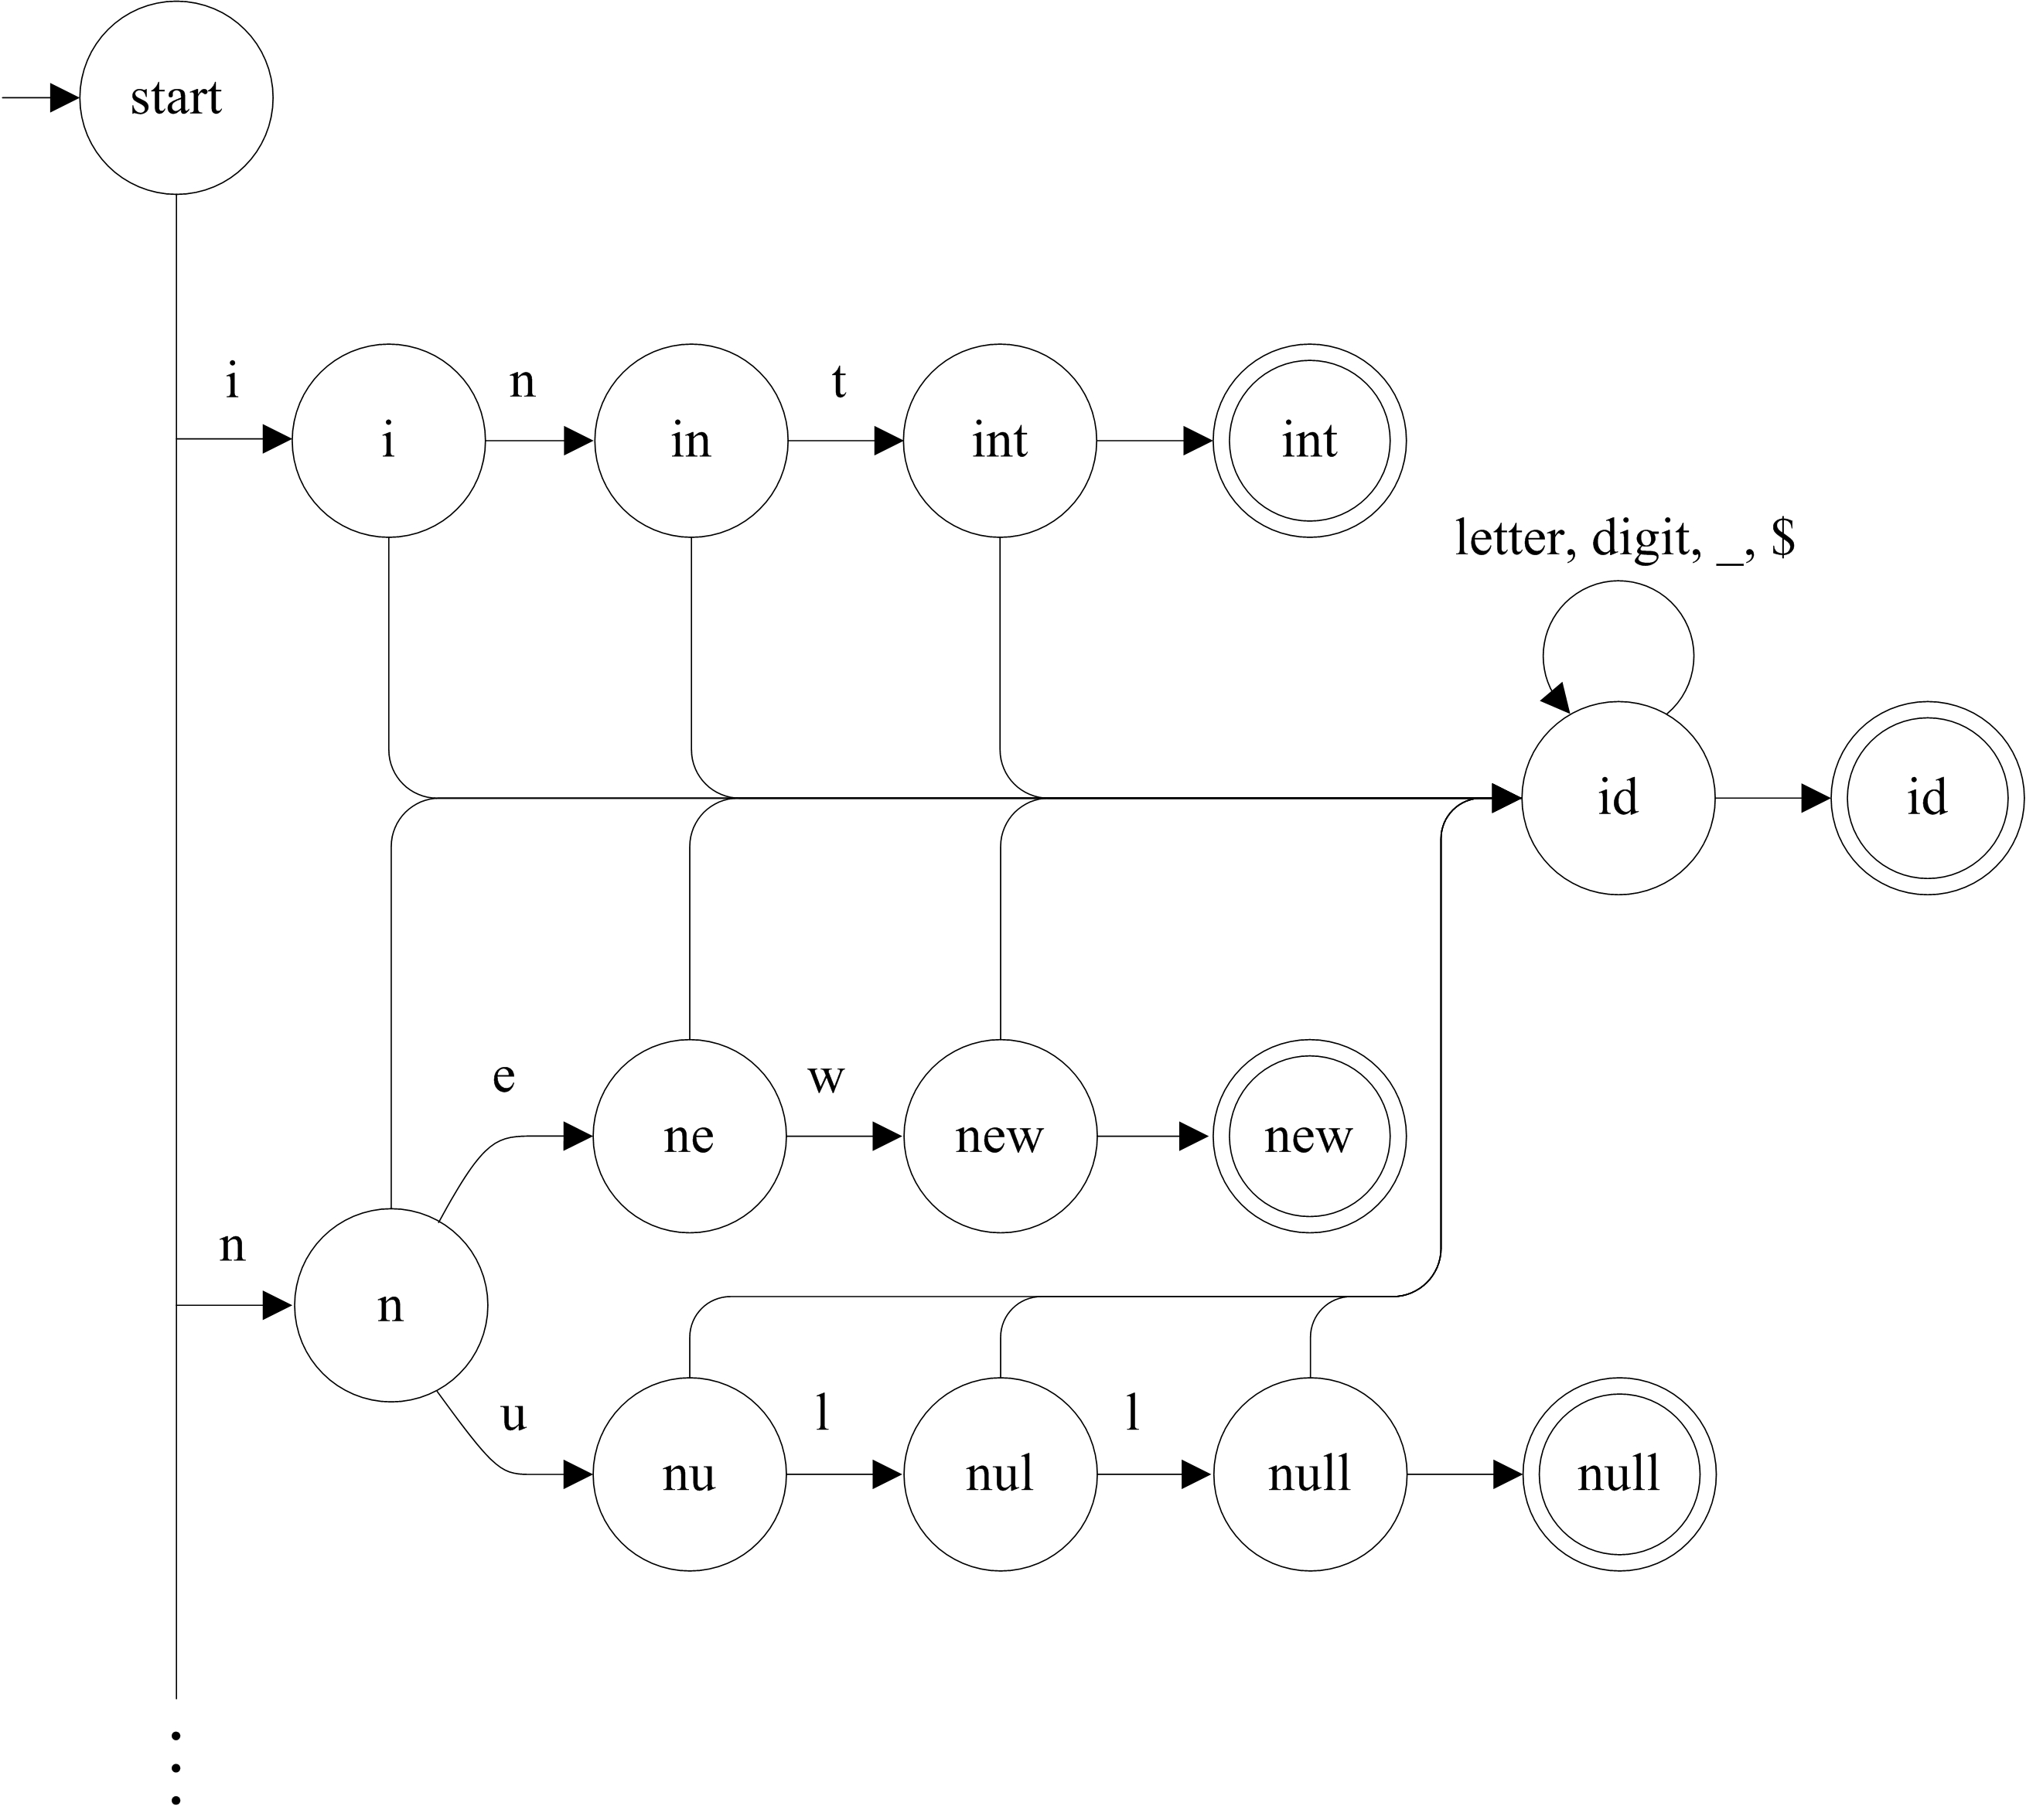
\includegraphics[scale=0.6]{{figures/figure02.02}.jpg}}
\end{center}
\end{frame}

\begin{frame}[fragile]
\pause

\begin{lstlisting}[language=Java]
...
else if (ch == 'n') {
    buffer.append(ch);
    nextCh();
    if (ch == 'e') {
        buffer.append(ch);
        nextCh();
        if (ch == 'w') {
            buffer.append(ch);
            nextCh();
            if (!isLetter(ch) && !isDigit(ch) && ch != '_' && ch !=  '$') {
                return new TokenInfo(NEW, line);
            }
        }
    }
    else if (ch == 'u') {
        buffer.append(ch);
        nextCh();
        if (ch == 'l') {
            buffer.append(ch);
            nextCh();
            if (ch == 'l') {
                buffer.append(ch);
                nextCh();
                if (!isLetter(ch) && !isDigit(ch) && ch != '_' && ch !=  '$') {
                    return new TokenInfo(NULL, line);
                }
            }
        }
    }
\end{lstlisting}
\end{frame}

\begin{frame}[fragile]
\pause

\begin{lstlisting}[language=Java]
    while (isLetter(ch) || isDigit(ch) || 
            ch == '_' || ch == '$') {
        buffer.append(ch);
        nextCh();
    }
    return new TokenInfo(IDENTIFIER, buffer.toString(), line);
}
else ...
\end{lstlisting}

\pause
\bigskip

A better approach for recognizing reserved words
\begin{center}
\visible<3->{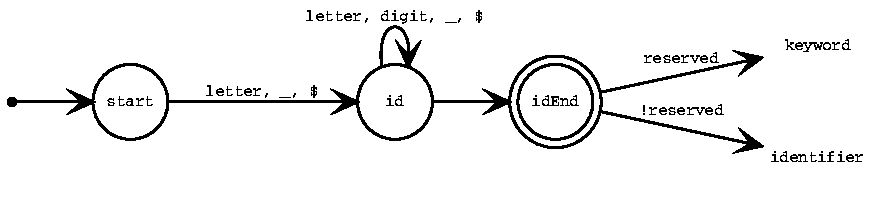
\includegraphics[scale=0.6]{{figures/figure02.03}.jpg}}
\end{center}
\end{frame}

\begin{frame}[fragile]
\pause

\begin{lstlisting}[language=Java]
    if (isLetter(ch) || ch == '_' || ch == '$') {
        buffer = new StringBuffer();
        while (isLetter(ch) || isDigit(ch) || 
               ch == '_' || ch == '$'){
            buffer.append(ch);
            nextCh();
        }
        String identifier = buffer.toString();                 
        if (reserved.containsKey(identifier)) {
            return new TokenInfo(reserved.get(identifier), line); 
        }
        else {                     
            return new TokenInfo(IDENTIFIER, identifier, line);                 
        }
    }
\end{lstlisting}

\pause
\bigskip

The above approach relies on a map (hash table), \lstinline{reserved}, mapping reserved identifiers to their representations:

\begin{lstlisting}[language=Java]
reserved = new Hashtable<String, Integer>();
reserved.put("abstract", ABSTRACT);  
reserved.put("boolean", BOOLEAN);         
reserved.put("char", CHAR);
...
reserved.put("while", WHILE);
\end{lstlisting}
\end{frame}

\begin{frame}[fragile]
\pause

A state transition diagram for separators and operators and the corresponding code
\begin{center}
\visible<2->{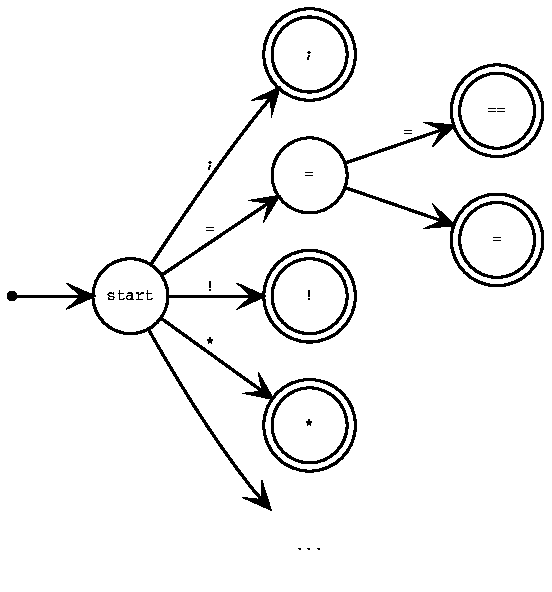
\includegraphics[scale=0.6]{{figures/figure02.04}.jpg}}
\end{center}
\end{frame}

\begin{frame}[fragile]
\pause

\begin{lstlisting}[language=Java]
switch (ch) {
...
case ';':
    nextCh();             
    return new TokenInfo(SEMI, line);         
case '=':             
    nextCh();             
    if (ch == '=') {                 
        nextCh();                 
        return new TokenInfo(EQUAL, line);             
    }             
    else {                 
        return new TokenInfo(ASSIGN, line);             
    }         
case '!':             
    nextCh();             
    return new TokenInfo(LNOT, line);         
case '*':             
    nextCh();             
    return new TokenInfo(STAR, line);
...
}
\end{lstlisting}
\end{frame}

\begin{frame}[fragile]
\pause

A state transition diagram for whitespace and the corresponding code
\begin{center}
\visible<2->{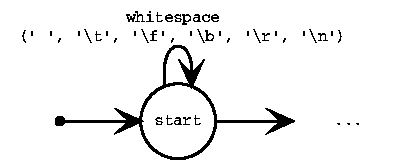
\includegraphics[scale=0.6]{{figures/figure02.05}.jpg}}
\end{center}

\begin{lstlisting}[language=Java]
while (isWhitespace(ch)) {                 
    nextCh();             
}
\end{lstlisting}
\end{frame}

\begin{frame}[fragile]
\pause

A state transition diagram for comments and the corresponding code
\begin{center}
\visible<2->{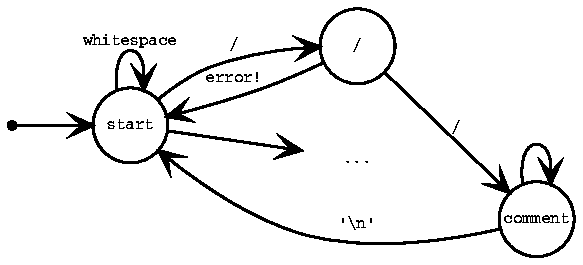
\includegraphics[scale=0.6]{{figures/figure02.06}.jpg}}
\end{center}
\end{frame}

\begin{frame}[fragile]
\pause

\begin{lstlisting}[language=Java]
boolean moreWhiteSpace = true;
while (moreWhiteSpace) {
    while (isWhitespace(ch)) {
        nextCh();
    }
    if (ch == '/') {
        nextCh();
        if (ch == '/') { 
            // CharReader maps all new lines to '\n'
            while (ch != '\n' && ch != EOFCH) {
                nextCh();
            }
        }
        else {
            reportScannerError("Operator / is not supported in j--.");
        }
    }
    else {
        moreWhiteSpace = false;
    }
}
\end{lstlisting}
\end{frame}

\section{Regular Expresssions}
\begin{frame}[fragile]
\pause

Regular expressions provide a simple notation for describing patterns of characters in a text

\pause
\bigskip

A regular expression defines a language of strings over an alphabet, and may take one of the following forms
\begin{enumerate}
\item If $a$ is in our alphabet, then the regular expression $a$ describes the language $L(a)$ consisting of the string $a$

\item If $r$ and $s$ are regular expressions then their concatenation $rs$ is also a regular expression describing the language $L(rs)$ of all possible strings obtained by concatenating a string in the language described by $r$, to a string in the language described by $s$

\item If $r$ and $s$ are regular expressions then the alternation $r|s$ is also a regular expression describing the language $L(r|s)$ consisting of all strings described by either $r$ or $s$

\item If $r$ is a regular expression, the repetition (aka the Kleene closure) $r*$ is also a regular expression describing the language $L(r*)$ consisting of strings obtained by concatenating zero or more instances of strings described by $r$ together

\item $\epsilon$ is a regular expression describing the language containing only the empty string

\item If $r$ is a regular expression, then $(r)$ is also a regular expression denoting the same language
\end{enumerate}
\end{frame}

\begin{frame}[fragile]
\pause

For example, given an alphabet $\{a,b\}$

\begin{enumerate}
\item $a(a|b)*$ denotes the language of non-empty strings of $a$'s and $b$'s, beginning with an $a$
\item $aa | ab | ba | bb$ denotes the language of all two-symbol strings over the alphabet
\item $(a|b)\!*\!ab$ denotes the language of all strings of $a$'s and $b$'s, ending in $ab$
\end{enumerate}

\pause
\bigskip

As another example, in a programming language such as Java
\begin{enumerate}
\item Reserved words may be described as \lstinline{abstract | boolean | char | ... | while}

\item Operators may be described as \lstinline{= | == | > | ... | *}

\item Identifiers may be described as \lstinline{([a-zA-Z] | _ | $)([a-zA-Z0-9] | _ | $)*}
\end{enumerate}
\end{frame}

\section{Finite State Automata}
\begin{frame}[fragile]
\pause

For any language described by a regular expression, there is a state transition diagram called Finite State Automaton that can parse strings in the language

\pause
\bigskip

A Finite State Automaton (FSA) $F$ is a quintuple $F = (\Sigma, S, s_0, M, F)$ where
\begin{itemize}
\item $\Sigma$ is the input alphabet
\item $S$ is a set of states
\item $s_0 \in S$ is a special start state
\item $M$ is a set of moves or state transitions of the form $$m(r, a) = s \text{ where } r,s \in S, a \in \Sigma$$ read as, ``if one is in state $r$, and the next input symbol is $a$, scan the $a$ and move into state $s$
\item $F \in S$ is a set of final states
\end{itemize}
\end{frame}

\begin{frame}[fragile]
\pause

For example, consider the regular expression $(a|b)a\!*\!b$ over the alphabet $\{a, b\}$ that describes the language consisting of all strings starting with either an $a$ or a $b$, followed by zero or more $a$'s, and ending with a $b$

\pause
\bigskip

An FSA $F$ that recognizes the language is $F = (\Sigma, S, s_0, M, F)$ where $\Sigma = \{a, b\}, S = \{0, 1, 2\}, s_0 = 0, M = \{m(0, a) = 1, m(0, b) = 1, m(1, a) = 1, m(1, b) = 2\}, F = \{2\}$

\pause
\bigskip

The corresponding transition diagram is shown below
\begin{center}
\visible<4->{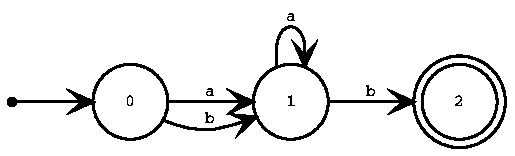
\includegraphics[scale=0.6]{{figures/figure02.07}.jpg}}
\end{center}
\end{frame}

\section{Non-deterministic (NFA) Versus Deterministic Finite State Automata (DFA)}
\begin{frame}[fragile]
\pause

A deterministic finite state automaton (DFA) is an automaton without $\epsilon$-moves, and there is a unique move from any state on an input symbol $a$, ie, there cannot be two moves $m(r, a) = s$ and $m(r, a) = t$, \noindent where $s \neq t$

\pause
\bigskip

A non-deterministic finite state automaton (NFA) is an automaton that allows either of the following
\begin{itemize}
\item More than one move from the same state, on the same input symbol $a$, ie, $m(r, a) = s$ and $m(r, a) = t$, \noindent where $s \neq t$

\item An $\epsilon$-move defined on the empty string $\epsilon$, ie, $m(r, \epsilon) = s$, which says we can move from state $r$ to state $s$ without scanning any input symbols
\end{itemize}
\end{frame}

\begin{frame}[fragile]
\pause

For example, an NFA that recognizes all strings of $a$'s and $b$'s that begin with an $a$ and end with a $b$ is $N = (\Sigma, S, s_0, M, F)$ where $\Sigma = \{a, b\}$, $S = \{0, 1, 2\}$, $s_0 = 0$, $M =  \{m(0, a) = 1, m(1, a) = 1, m(1, b) = 1, m(1, \epsilon) = 0, m(1, b) = 2\}$ and, $F = \{2\}$

\pause
\bigskip

The corresponding transition diagram is shown below
\begin{center}
\visible<3->{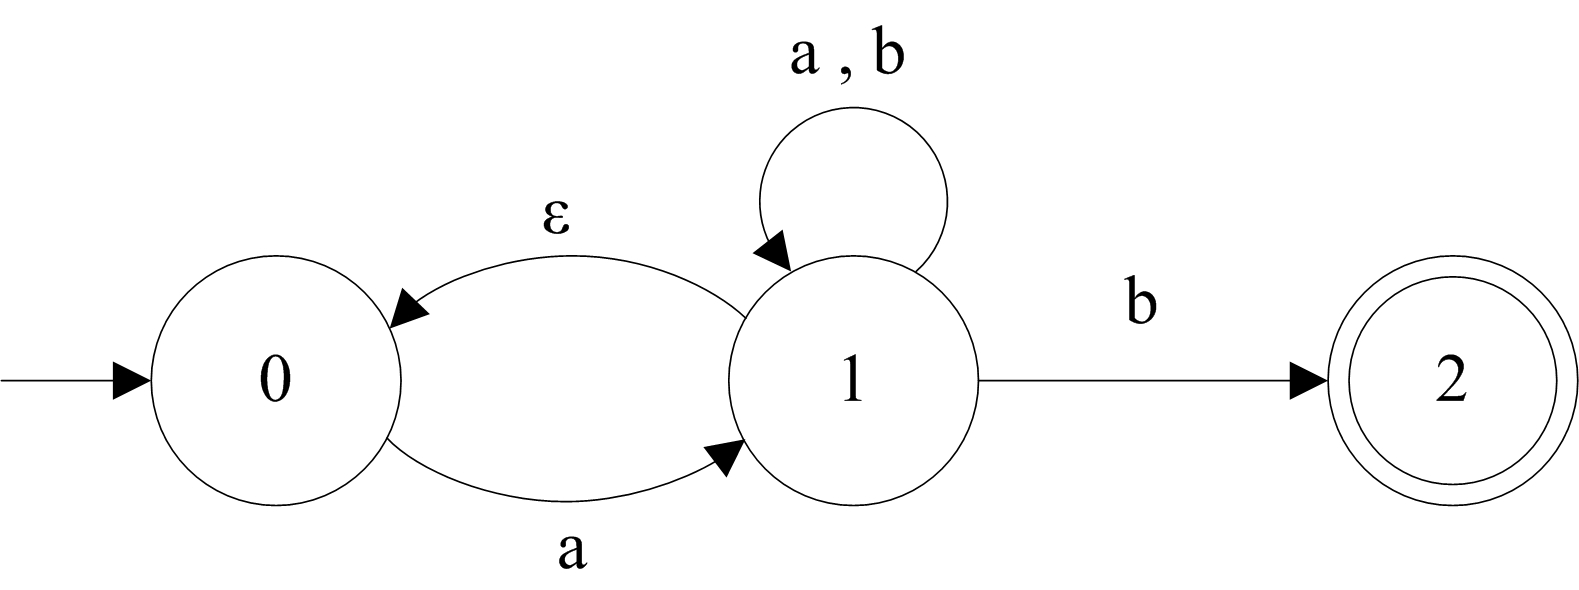
\includegraphics[scale=0.6]{{figures/figure02.08}.jpg}}
\end{center}

\pause
\bigskip

An NFA is said to recognize an input string if, starting in the start state, there exists a set of moves based on the input that takes us into one of the final states
\end{frame}

\section{Regular Expresssions to NFA}
\begin{frame}[fragile]
\pause

Given any regular expression $r$, we can construct (using Thompson's construction procedure) an NFA $N$ that recognizes the same language; ie, $L(N) = L(r)$

\pause
\bigskip

(Rule 1) If the regular expression $r$ takes the form of an input symbol, $a$, then the NFA that recognizes it has two states: a start state and a final state, and a move on symbol $a$ from the start state to the final state

\begin{center}
\visible<3->{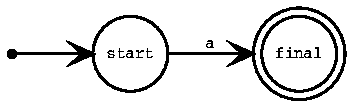
\includegraphics[scale=0.6]{{figures/figure02.09}.jpg}}
\end{center}

\pause
\bigskip

(Rule 2) If $N_r$ and $N_s$ are NFA recognizing the languages described by the regular expressions $r$ and $s$ respectively, then we can create a new NFA recognizing the language described by $rs$ as follows: we define an $\epsilon$-move from the final state of $N_r$  to the start state of $N_s$, then choose the start state of $N_r$ to be our new start state, and the final state of $N_s$ to be our new final state

\begin{center}
\visible<4->{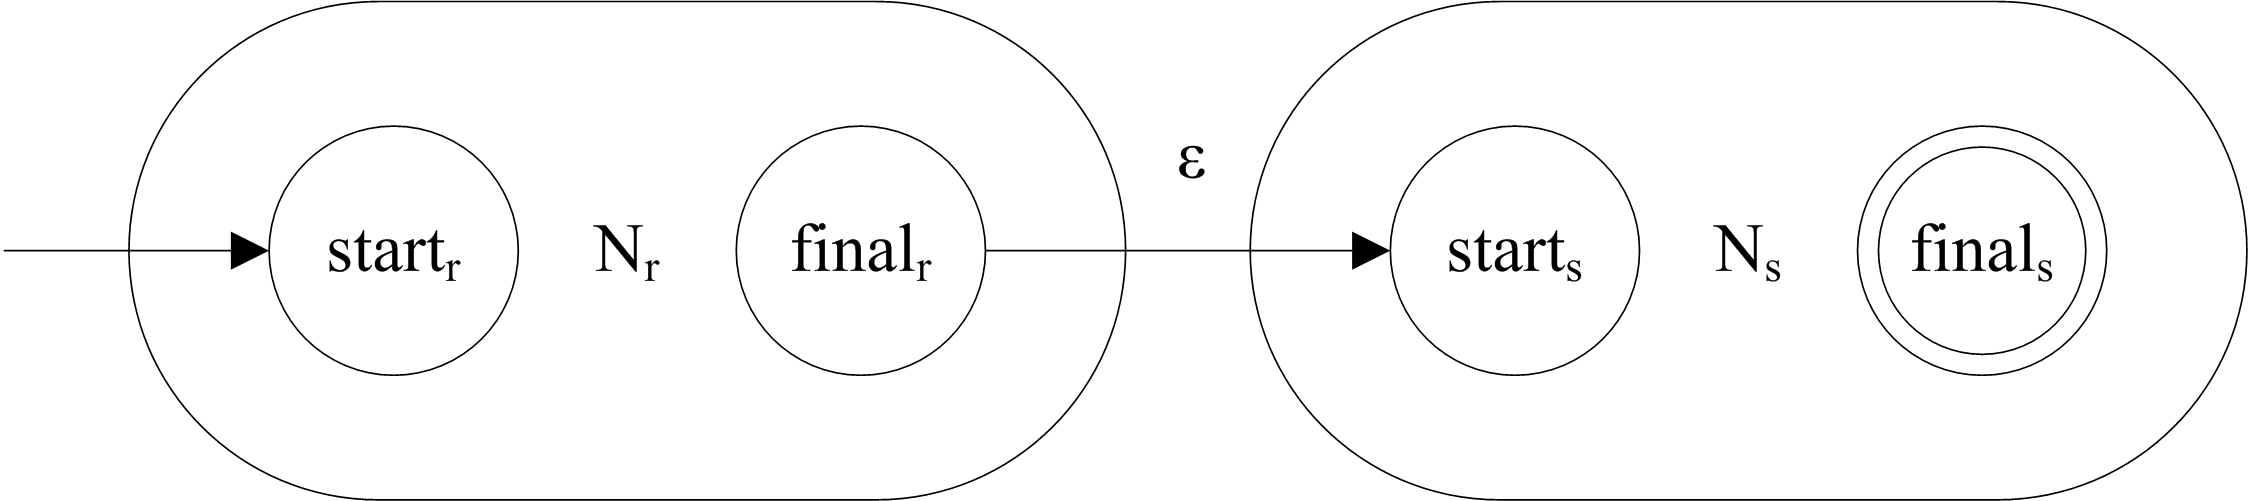
\includegraphics[scale=0.6]{{figures/figure02.10}.jpg}}
\end{center}
\end{frame}

\begin{frame}[fragile]
\pause

(Rule 3) If $N_r$ and $N_s$ are NFA recognizing the languages described by the regular expressions $r$ and $s$ respectively, then we can create a new NFA recognizing the language described by $r|s$ as follows: we define a new start state, having $\epsilon$-moves to each of the start states of $N_r$ and $N_s$, and we define a new final state and add $\epsilon$-moves from each of the final states of $N_r$ and $N_s$ to this state

\begin{center}
\visible<2->{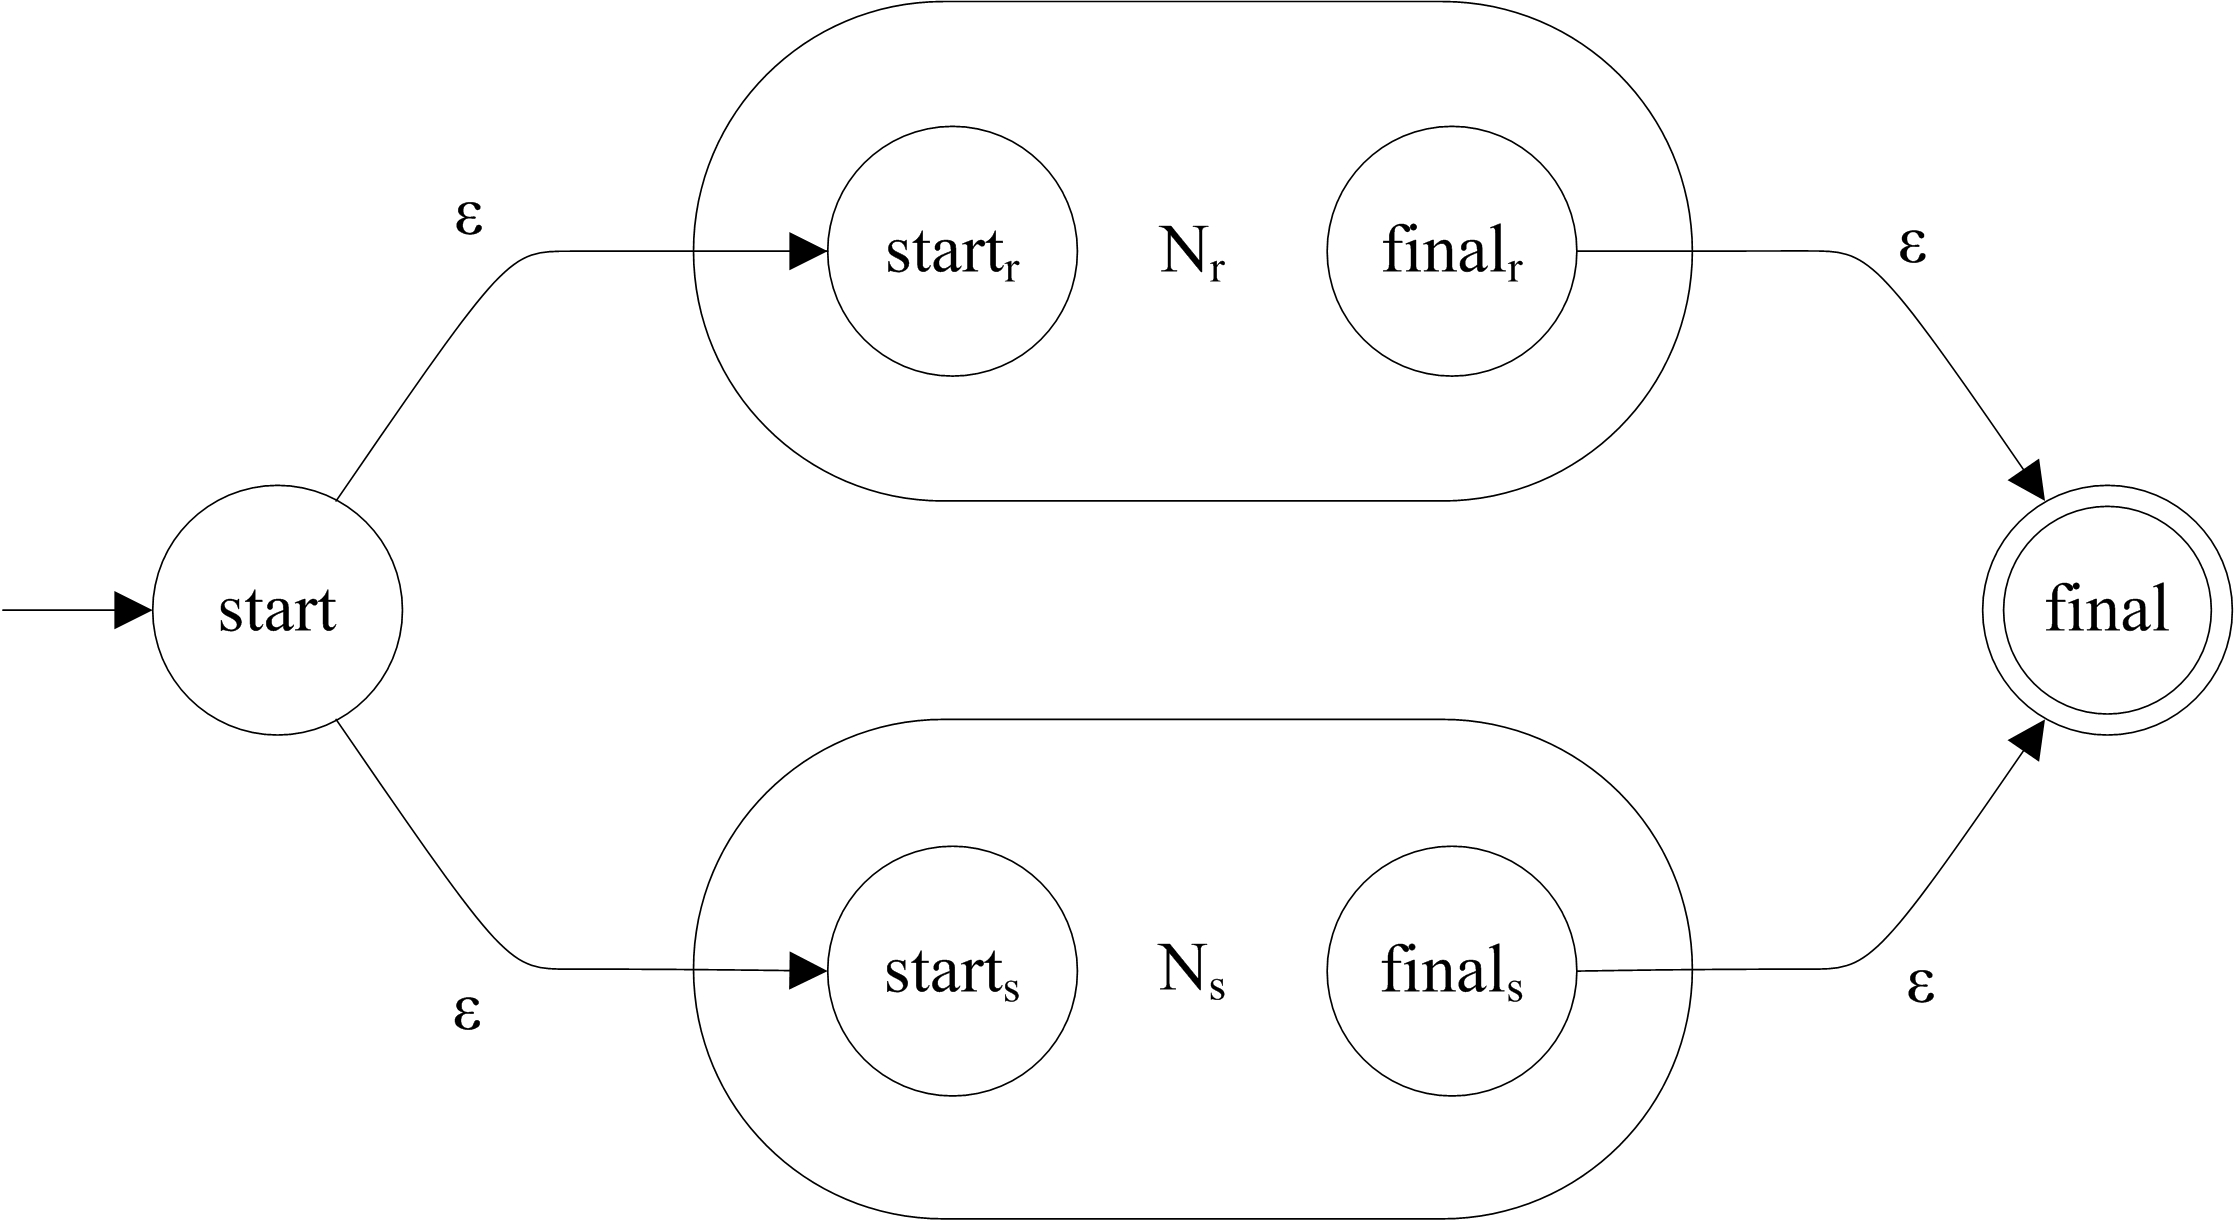
\includegraphics[scale=0.6]{{figures/figure02.11}.jpg}}
\end{center}
\end{frame}

\begin{frame}[fragile]
\pause

(Rule 4) If $N_r$ is an NFA recognizing that language described by a regular expression $r$, then we construct a new NFA recognizing $r*$ as follows:  we add an $\epsilon$-move from $N_r$'s final state back to its start state, define a new start state and a new final state, add $\epsilon$-moves from the new start state to both $N_r$'s start state and the new final state, and define an $\epsilon$-move from $N_r$'s final state to the new final state

\begin{center}
\visible<2->{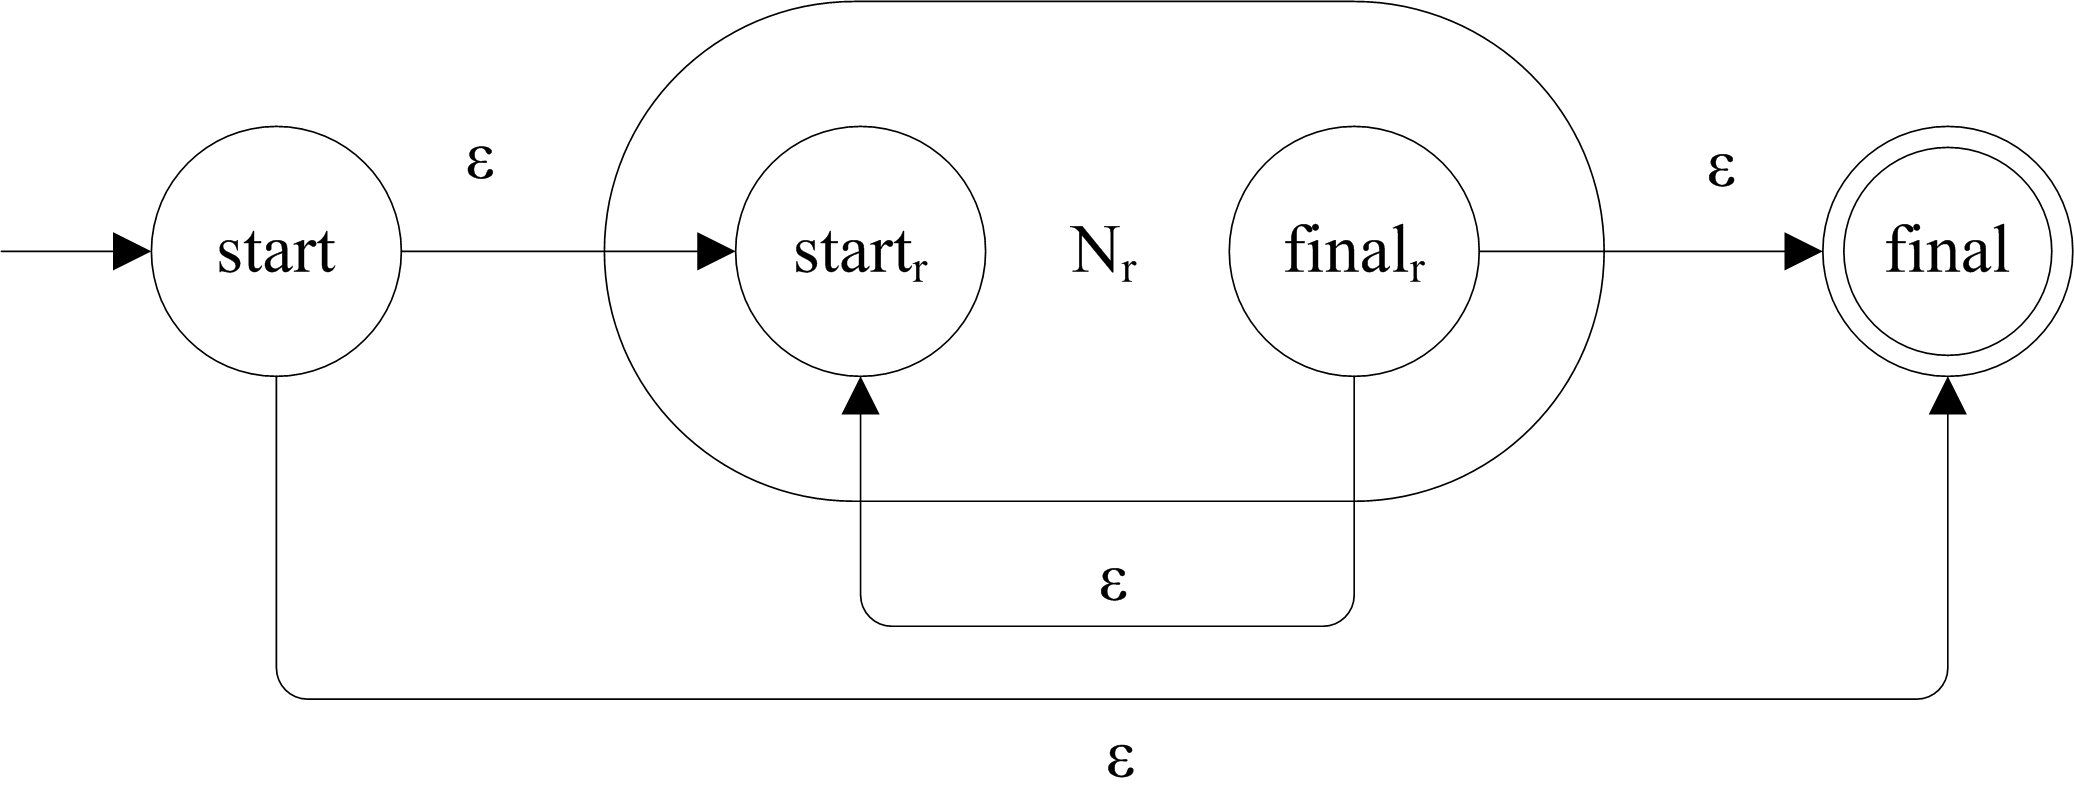
\includegraphics[scale=0.6]{{figures/figure02.12}.jpg}}
\end{center}

\pause
\bigskip

(Rule 5) If $r$ is $\epsilon$ then we just need an $\epsilon$-move from the start state to the final state

\begin{center}
\visible<3->{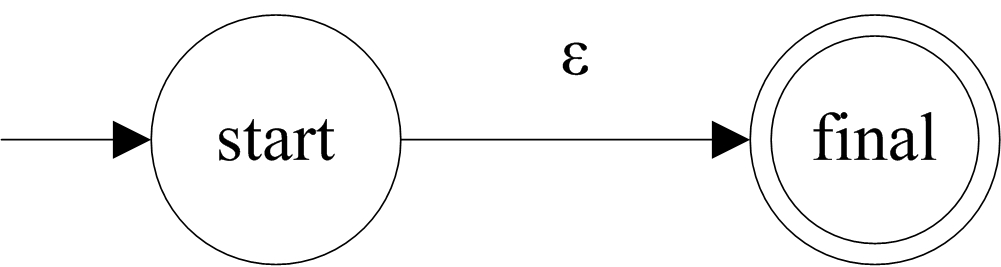
\includegraphics[scale=0.6]{{figures/figure02.13}.jpg}}
\end{center}

\pause
\bigskip

(Rule 6) If $N_r$ is our NFA recognizing the language described by $r$, then $N_r$ also recognizes the language described by $(r)$
\end{frame}

\begin{frame}[fragile]
\pause

As an example, let's construct an NFA for the regular expression $(a|b)a\!*\!b$, which has the following syntactic structure

\begin{center}
\visible<2->{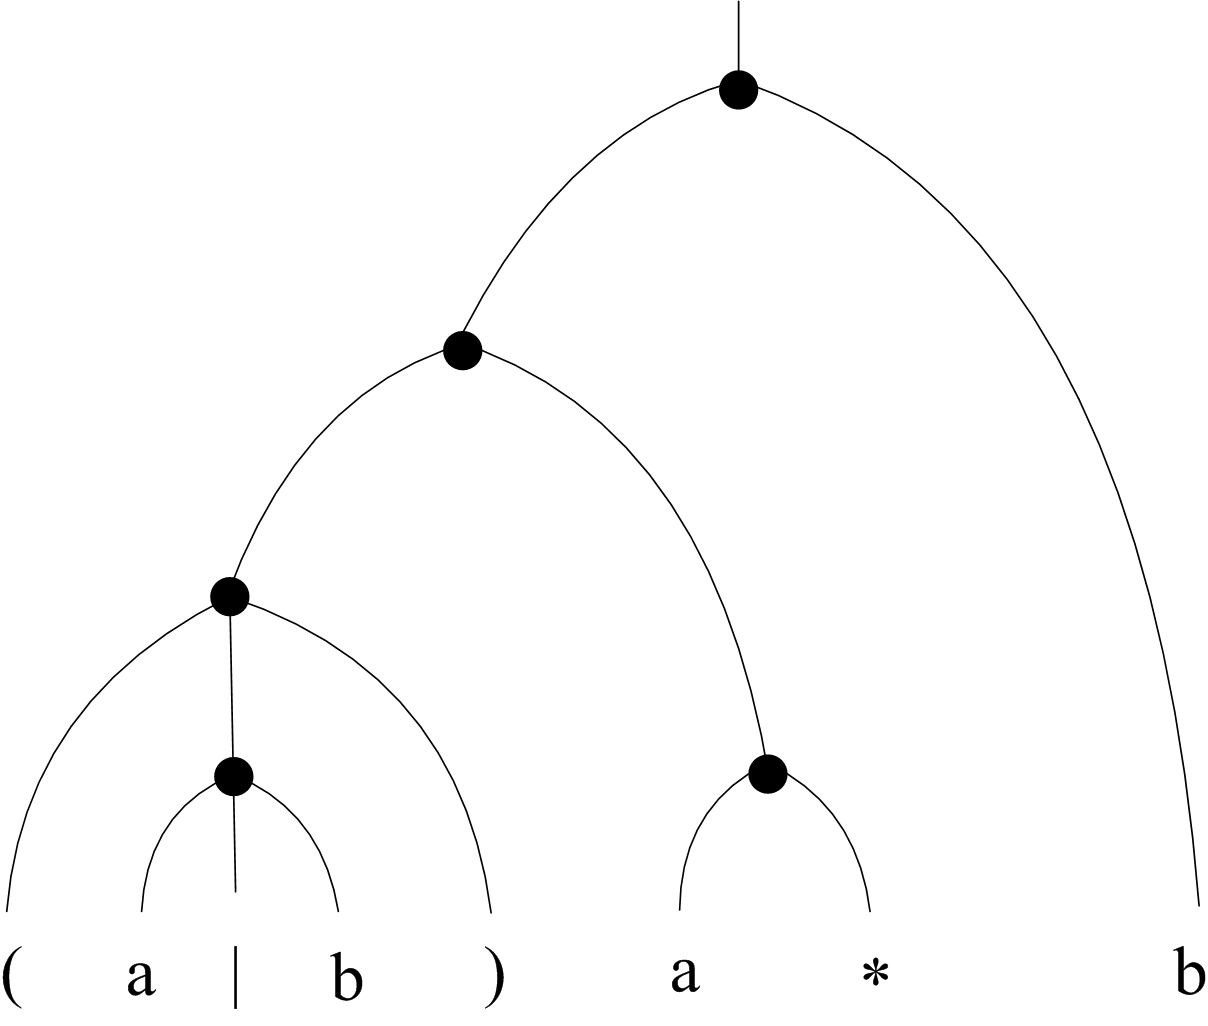
\includegraphics[scale=0.6]{{figures/figure02.14}.jpg}}
\end{center}

\pause
\bigskip

We start with the first $a$ and $b$; the automata recognizing these are easy enough to construct using Rule 1

\begin{center}
\visible<3->{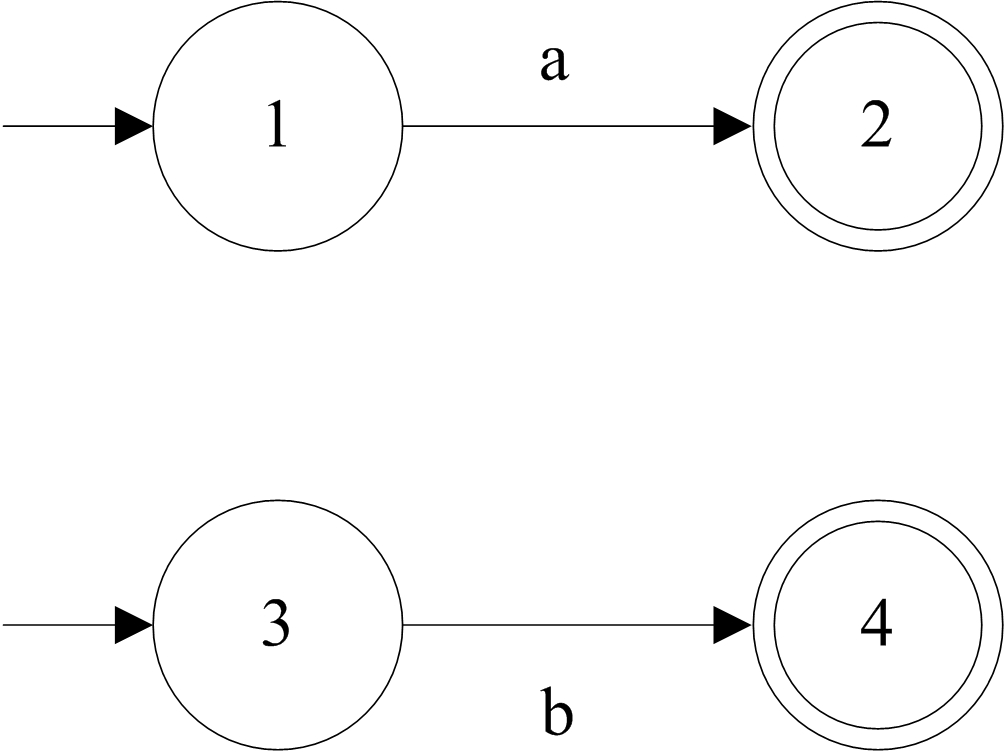
\includegraphics[scale=0.6]{{figures/construction-a1}.jpg}}
\end{center}
\end{frame}

\begin{frame}[fragile]
\pause

We then put them together using Rule 3 to produce an NFA recognizing $a|b$

\begin{center}
\visible<2->{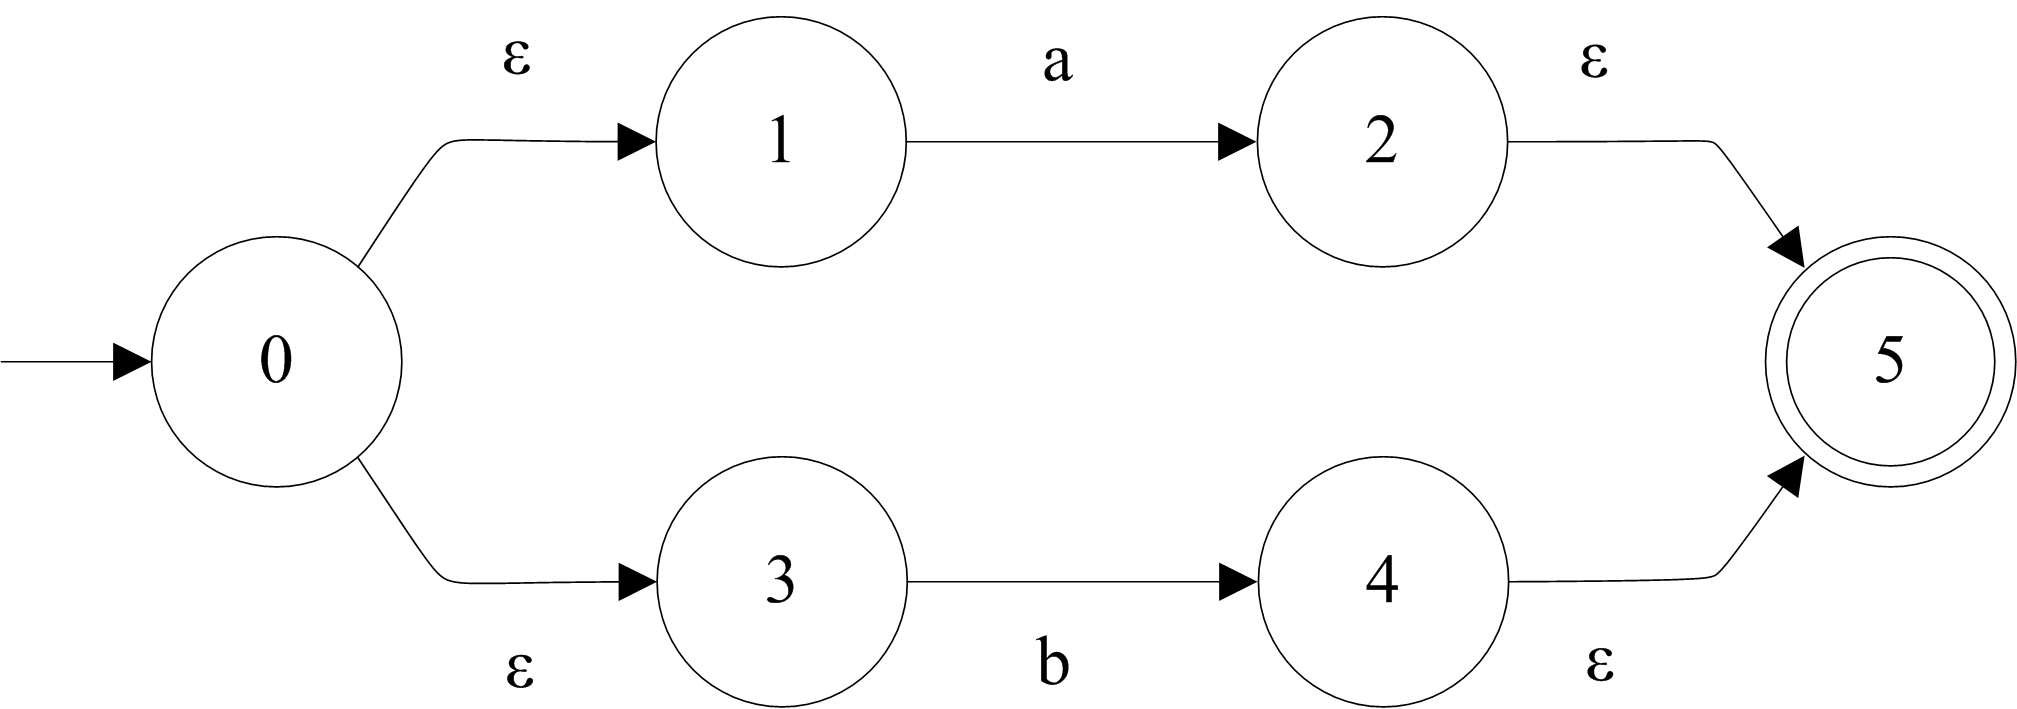
\includegraphics[scale=0.6]{{figures/construction-a2}.jpg}}
\end{center}

\pause
\bigskip

The NFA recognizing $(a|b)$ is the same as that recognizing $a|b$, by Rule 6

\pause
\bigskip

An NFA recognizing the second instance of $a$ is simple enough, by Rule 1 again

\begin{center}
\visible<4->{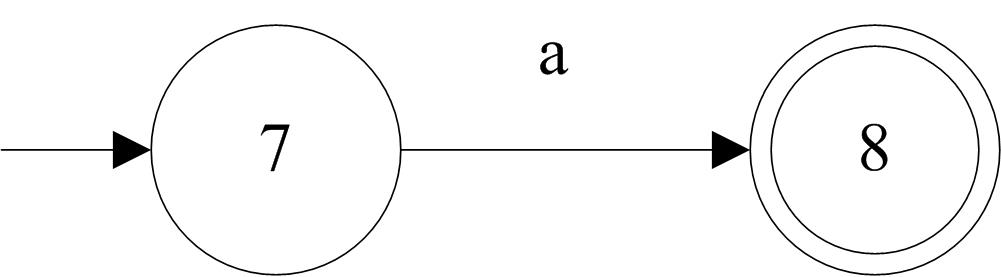
\includegraphics[scale=0.6]{{figures/construction-a3}.jpg}}
\end{center}

\pause
\bigskip

The NFA recognizing $a*$ can be constructed from the NFA for $a$, by applying Rule 4

\begin{center}
\visible<5->{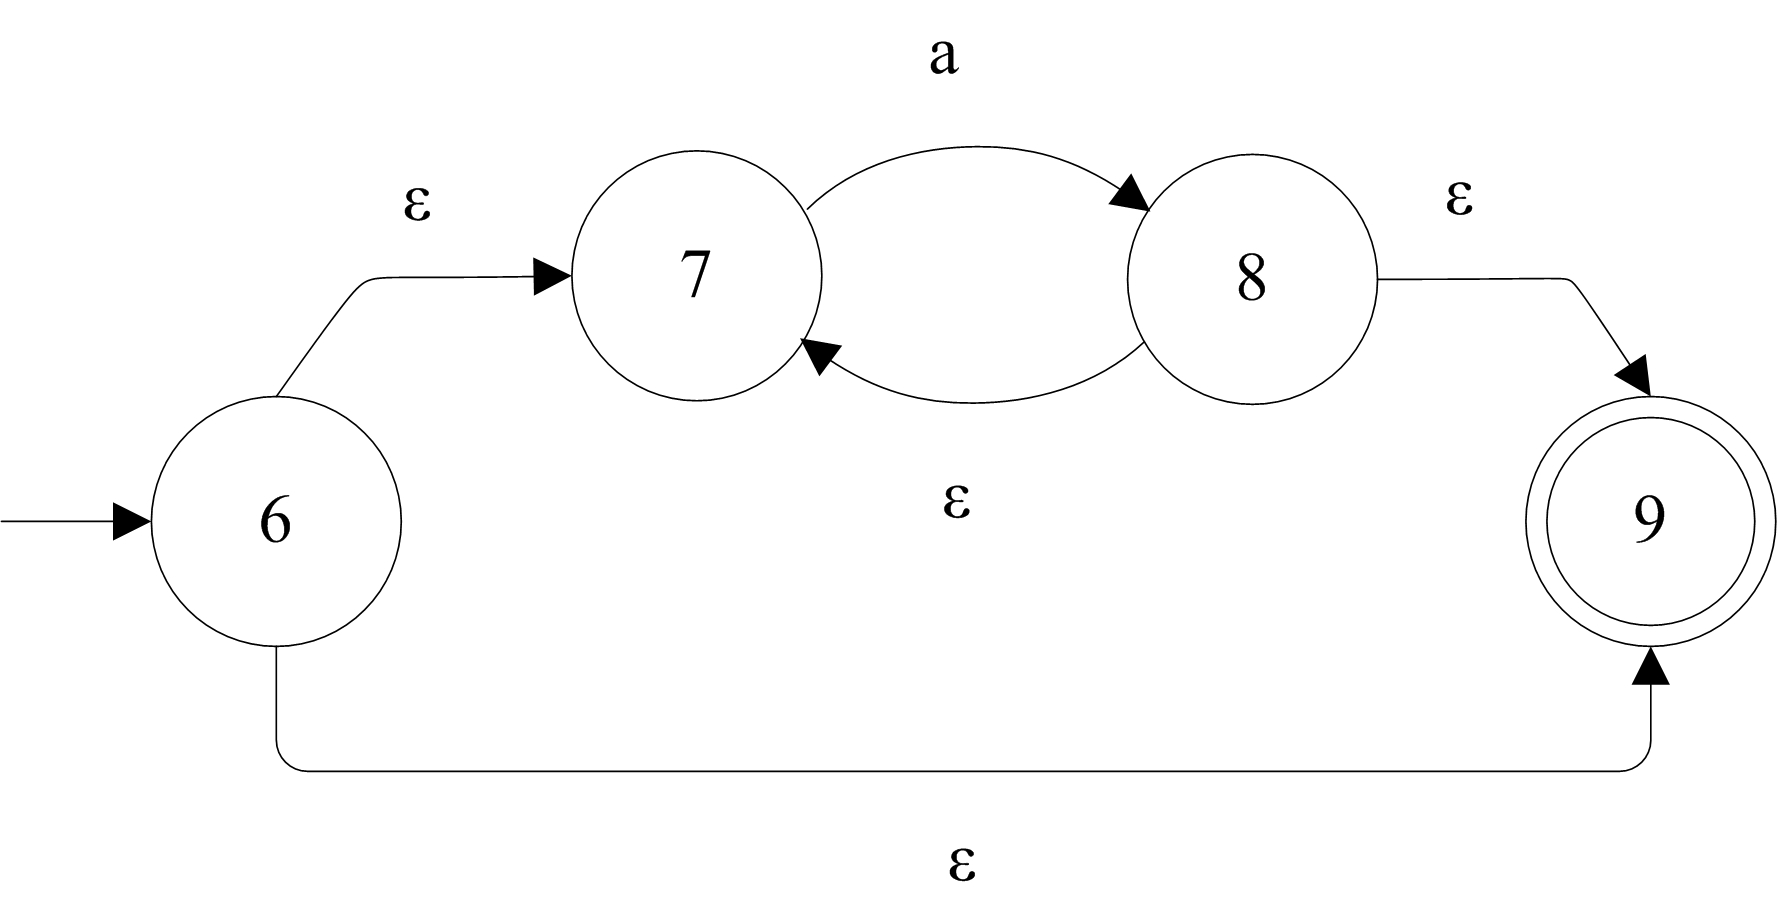
\includegraphics[scale=0.6]{{figures/construction-a4}.jpg}}
\end{center}
\end{frame}

\begin{frame}[fragile]
\pause

We then apply Rule 2 to construct an NFA recognizing the concatenation $(a|b)a*$

\begin{center}
\visible<2->{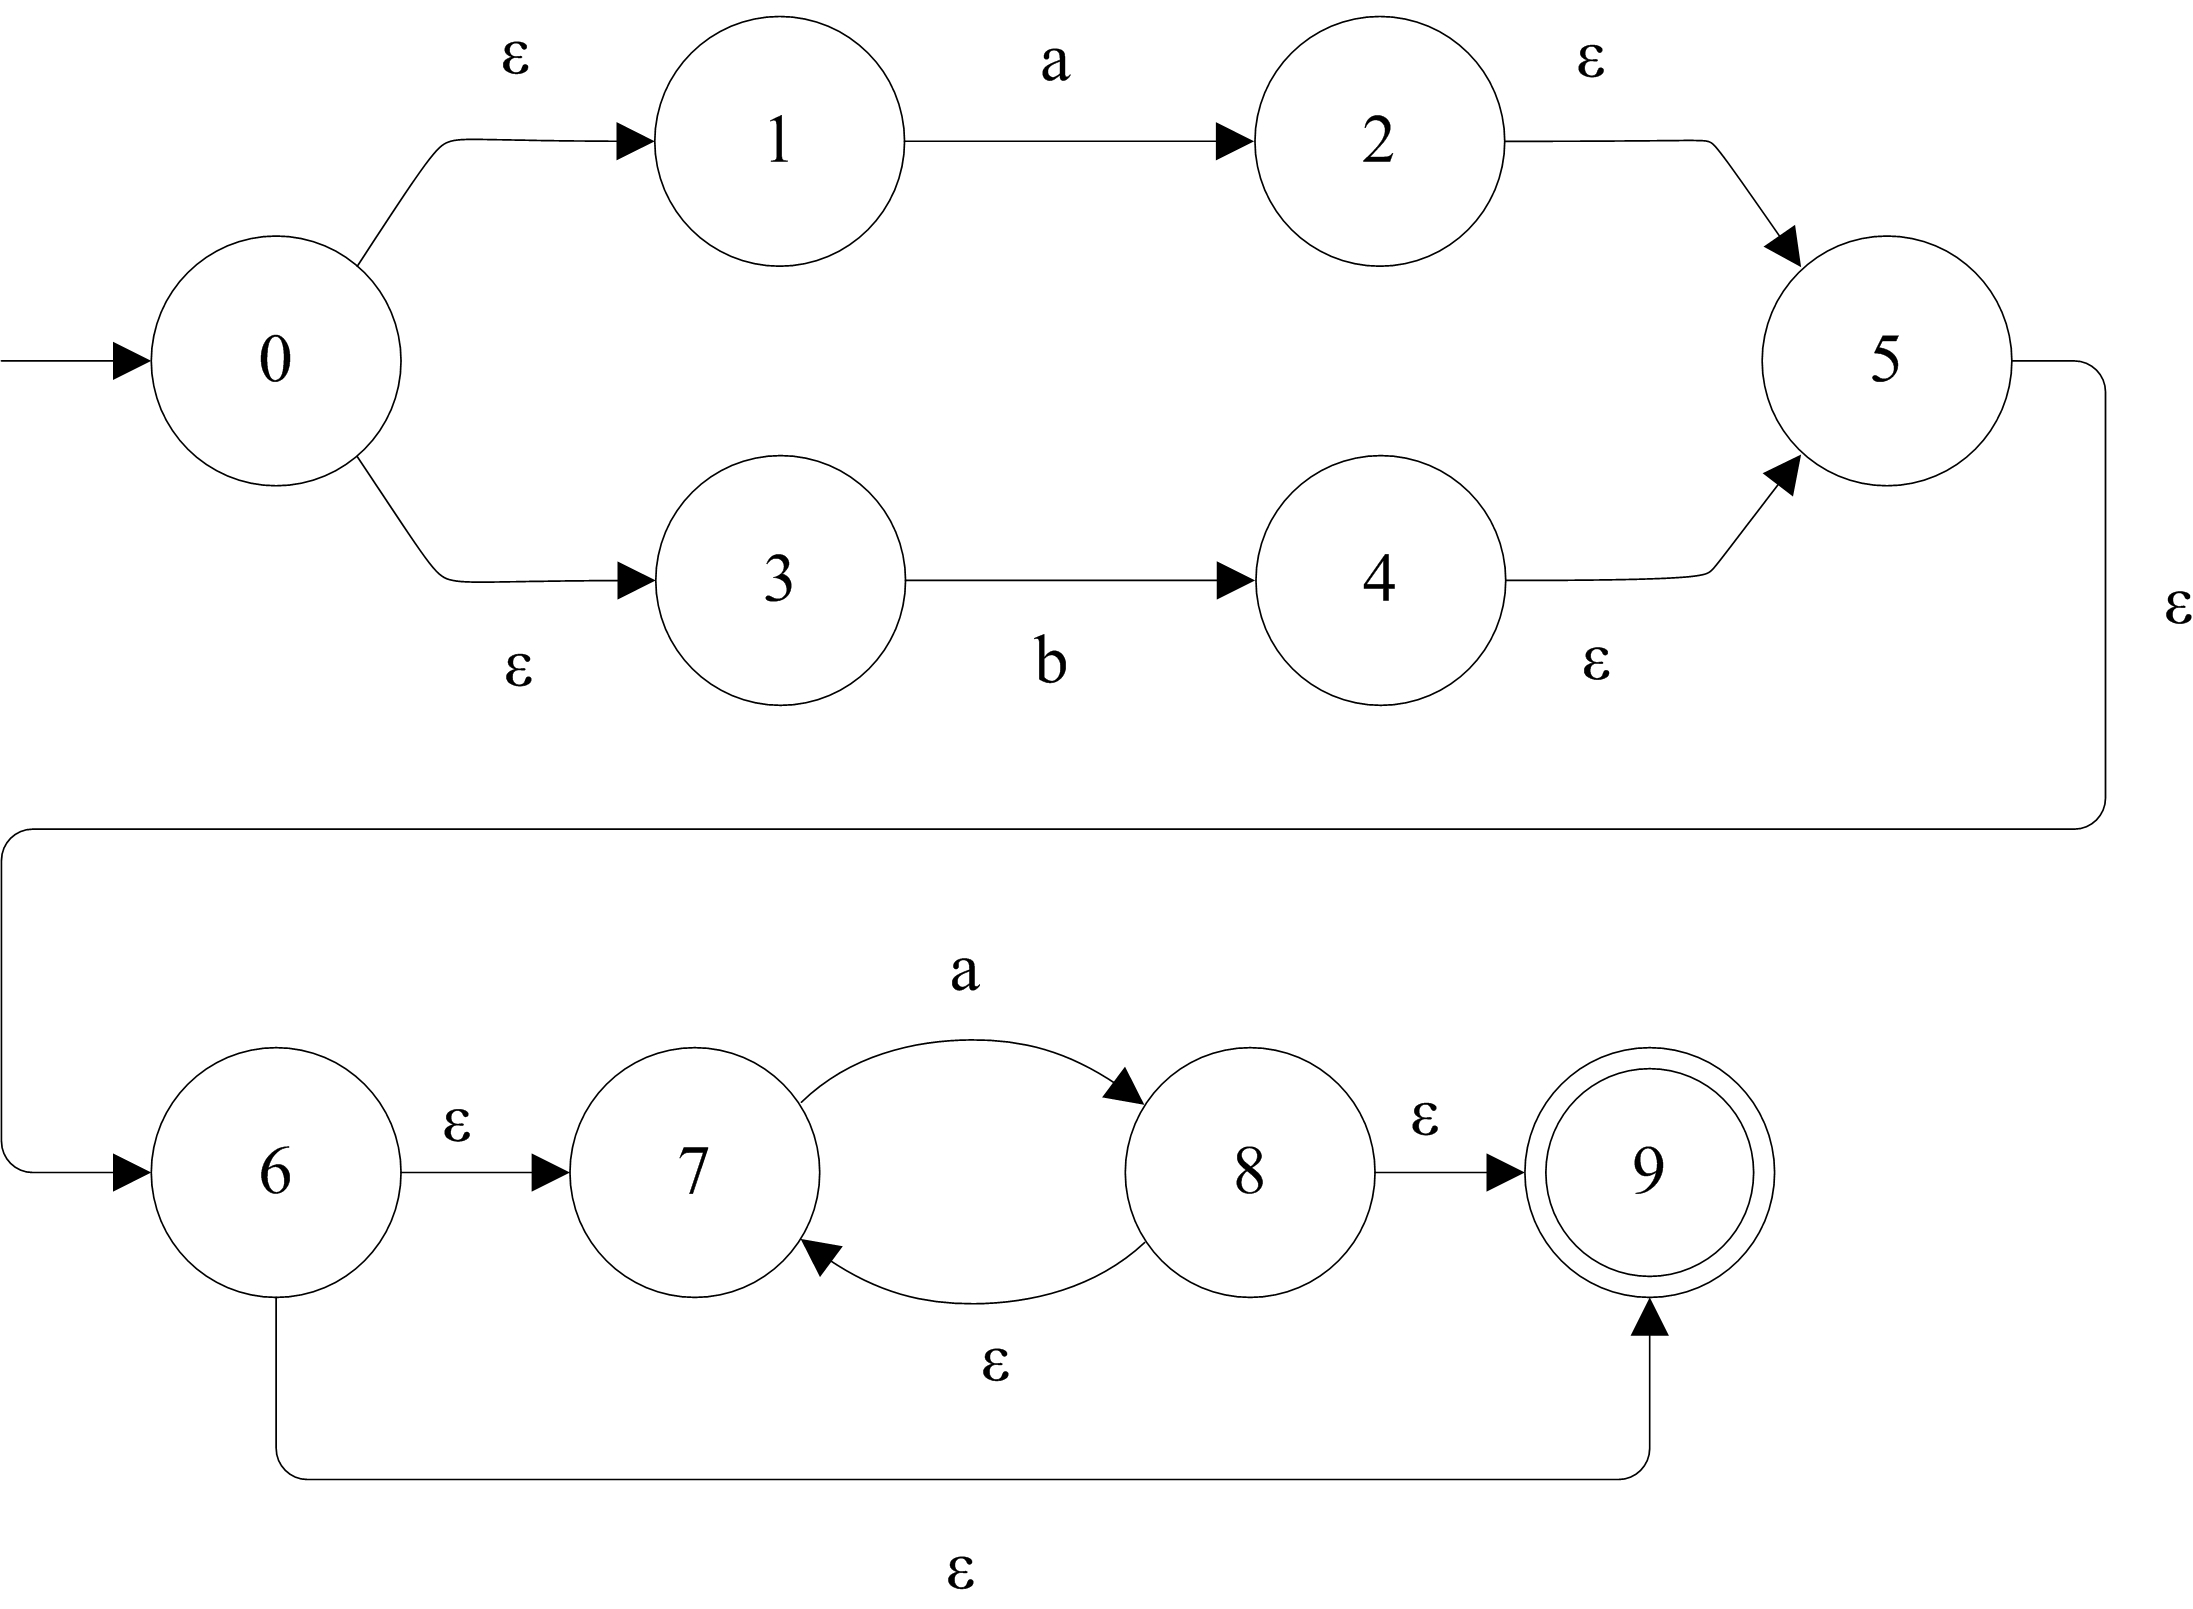
\includegraphics[scale=0.6]{{figures/construction-a5}.jpg}}
\end{center}
\end{frame}

\begin{frame}[fragile]
\pause

An NFA recognizing the second instance of $b$ is simple enough, by Rule 1 again

\begin{center}
\visible<2->{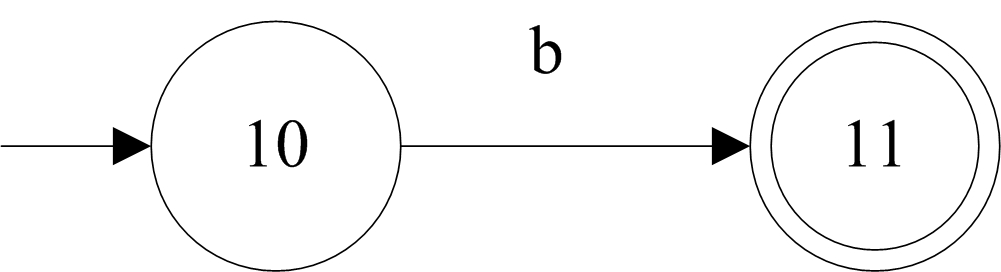
\includegraphics[scale=0.6]{{figures/construction-a6}.jpg}}
\end{center}

\pause
\bigskip

Finally, we can apply Rule 2 again to produce an NFA recognizing $(a|b)a\!*\!b$

\begin{center}
\visible<3->{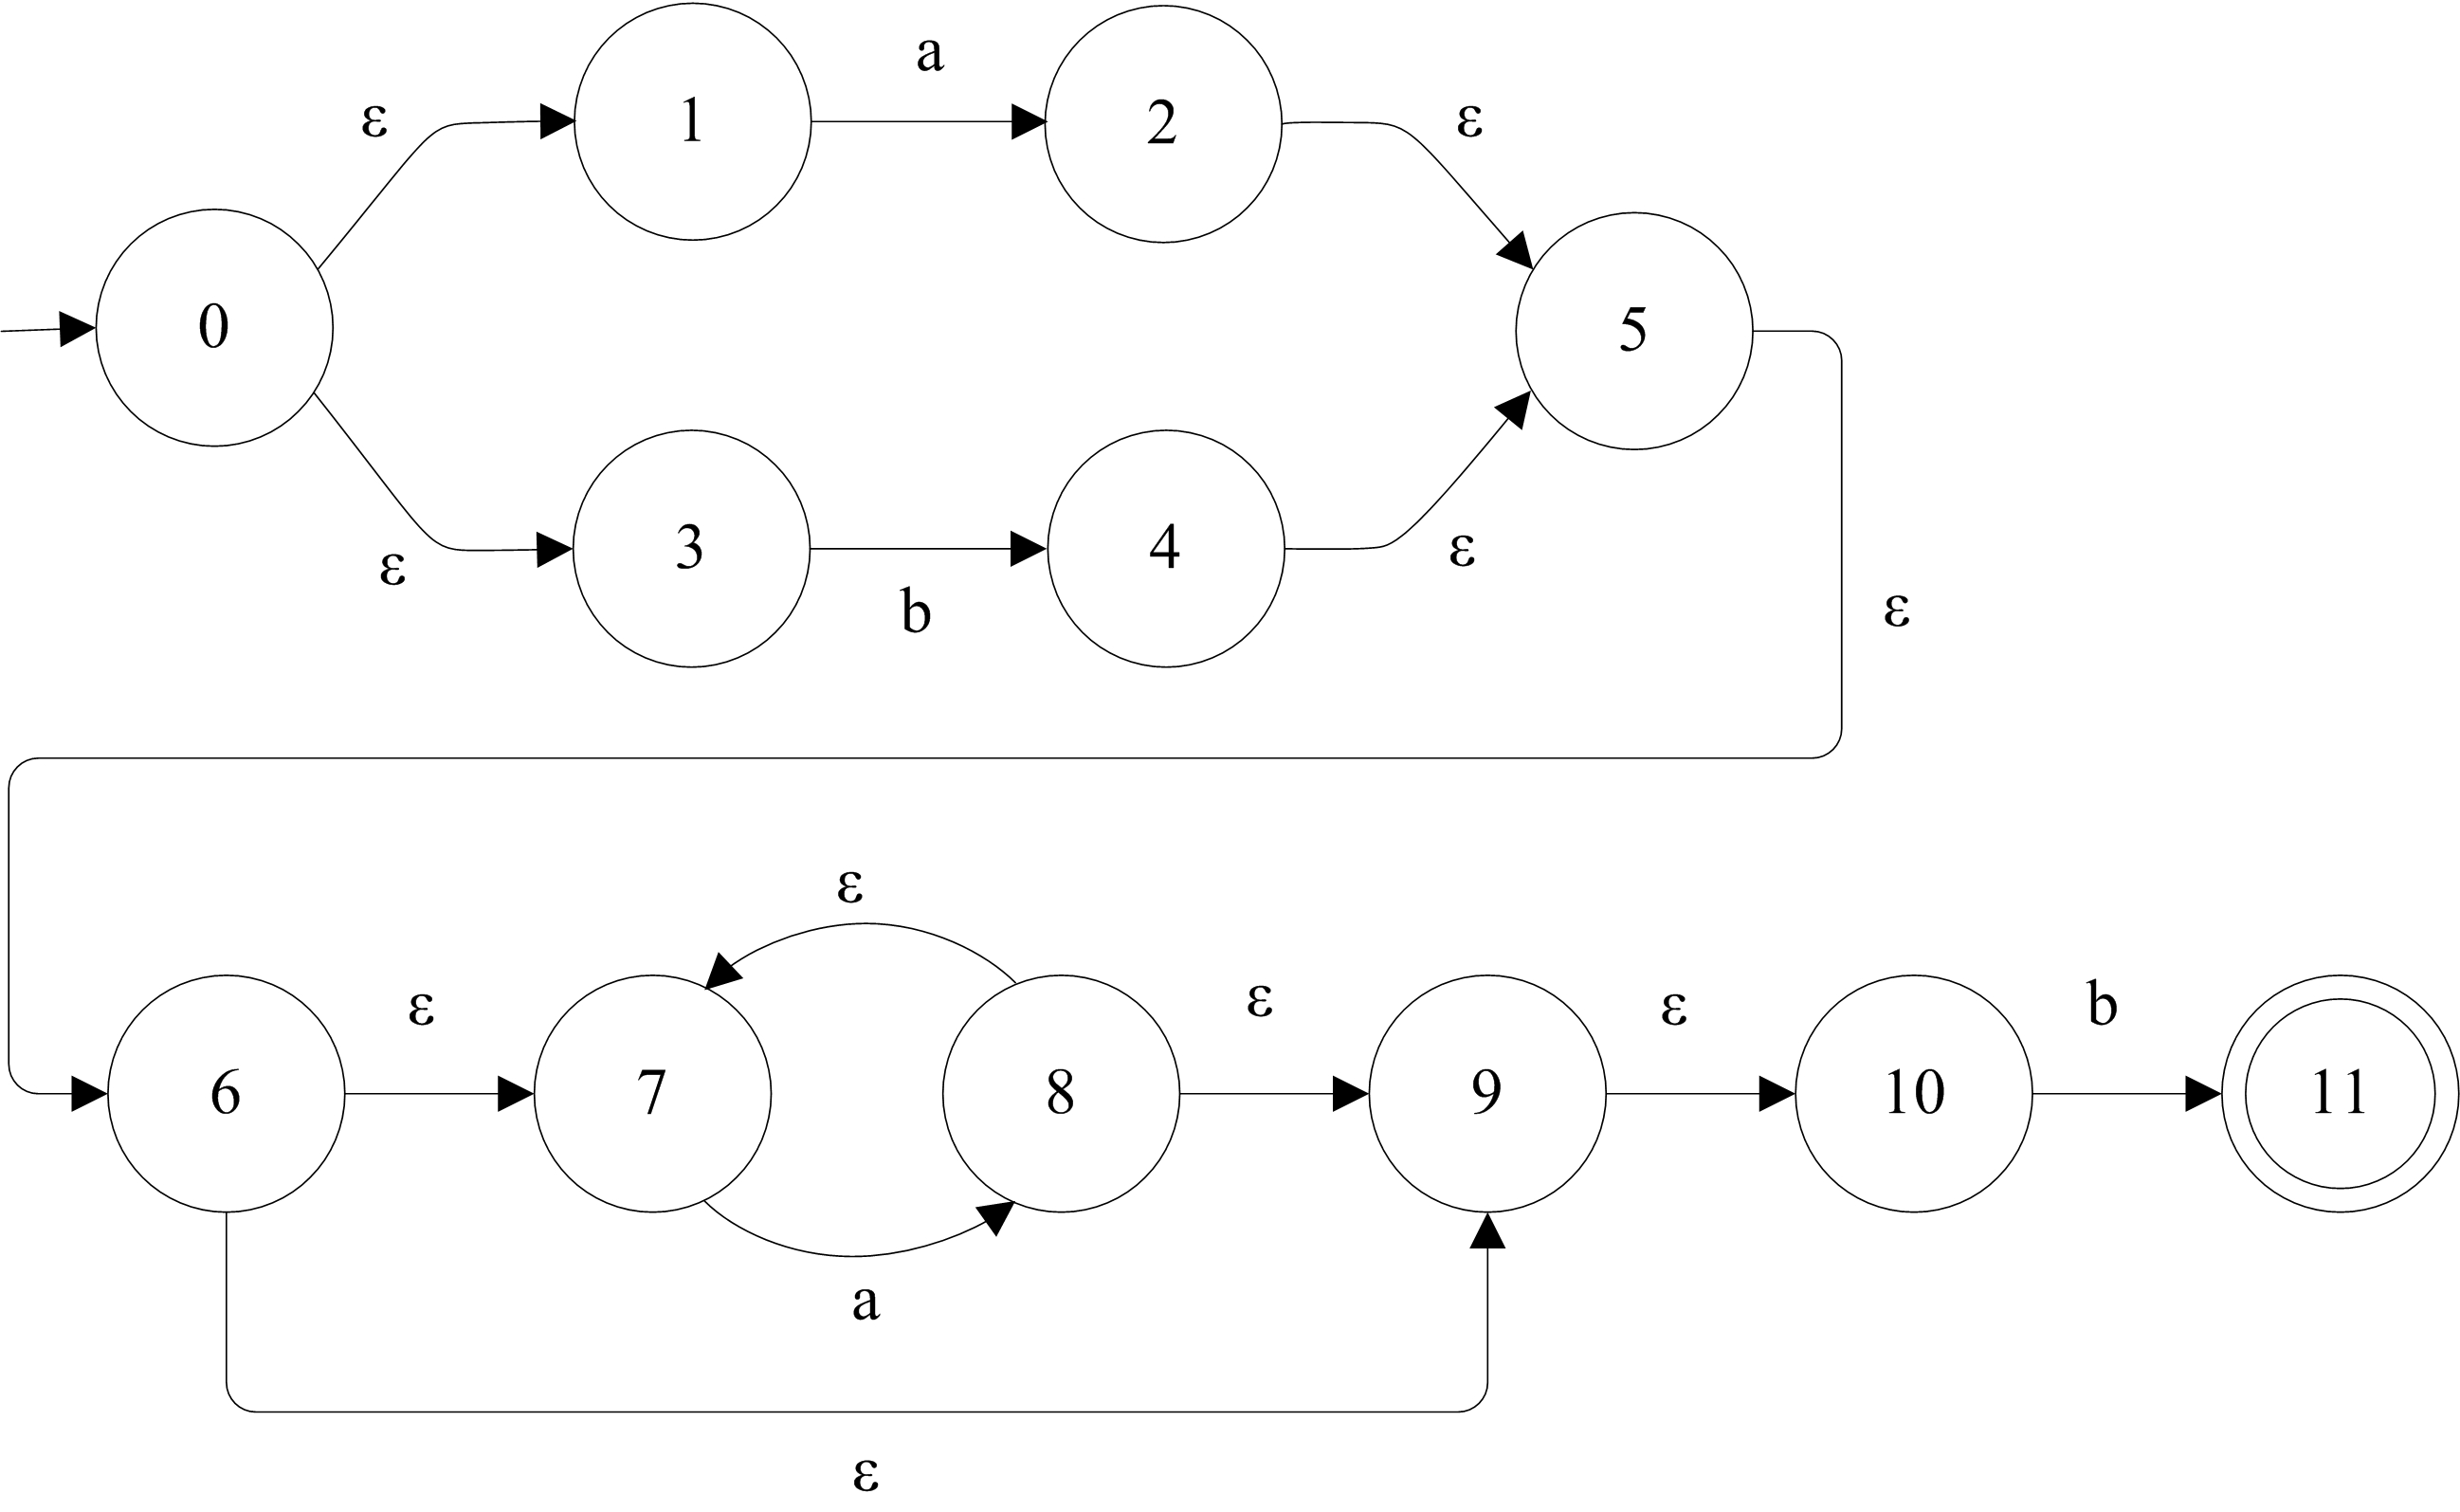
\includegraphics[scale=0.6]{{figures/figure02.15}.jpg}}
\end{center}
\end{frame}

\section{NFA to DFA}
\begin{frame}[fragile]
\pause

For any NFA, there is an equivalent DFA that can be constructed using the powerset (or subset) construction procedure

\pause
\bigskip

The DFA that we construct is always in a state that simulates all the possible states that the NFA could possibly be in having scanned the same portion of the input

\pause
\bigskip

The computation of all states reachable from a given state $s$ based on $\epsilon$-moves alone is called taking the $\epsilon$-closure of that state

\pause
\bigskip

The $\epsilon$-closure$(s)$ for a state $s$ includes $s$ and all states reachable from $s$ using $\epsilon$-moves alone, ie, $\epsilon$-closure$(s) = \{s\} \cup \{r \in S | \text{ there is a path of only } \epsilon\text{-moves from } s \text{ to } r\}$

\pause
\bigskip

The $\epsilon$-closure$(S)$ for a set of states $S$ includes $S$ and all states reachable from any state $s \in S$ using  $\epsilon$-moves alone
\end{frame}

\begin{frame}[fragile]
\pause

\begin{algorithm}[H]
\begin{algorithmic}
\REQUIRE a set of states, $S$
\ENSURE $\epsilon$-closure($S$)
\STATE {Stack $P$.addAll($S$)}   \COMMENT{a stack containing all states in $S$}
\STATE {Set $C$.addAll($S$)}     \COMMENT{the closure initially contains the states in $S$}
\WHILE {! $P$.empty()}
\STATE $s$ $\gets$ $P$.pop()
\FOR {$r$ in $m(s, \epsilon)$}
\STATE{} \COMMENT{$m(s, \epsilon)$ is a set of states}
\IF {$r \notin C$}
\STATE $P$.push($r$)
\STATE $C$.add($r$)
\ENDIF
\ENDFOR
\ENDWHILE
\RETURN $C$
\end{algorithmic}
\caption{$\epsilon$-closure($S$) for a Set of States $S$}
\end{algorithm}

\pause
\bigskip

\begin{algorithm}[H]
\begin{algorithmic}
\REQUIRE a state, $s$
\ENSURE $\epsilon$-closure($s$)
\STATE {Set $S$.add($s$)}  \COMMENT{$S = \{s\}$}
\RETURN $\epsilon$-closure($S$)
\end{algorithmic}
\caption{$\epsilon$-closure($s$) for a State $s$}
\end{algorithm}
\end{frame}

\begin{frame}[fragile]
\pause

NFA for the regular expression $(a|b)a\!*\!b$ from before
\begin{center}
\visible<2->{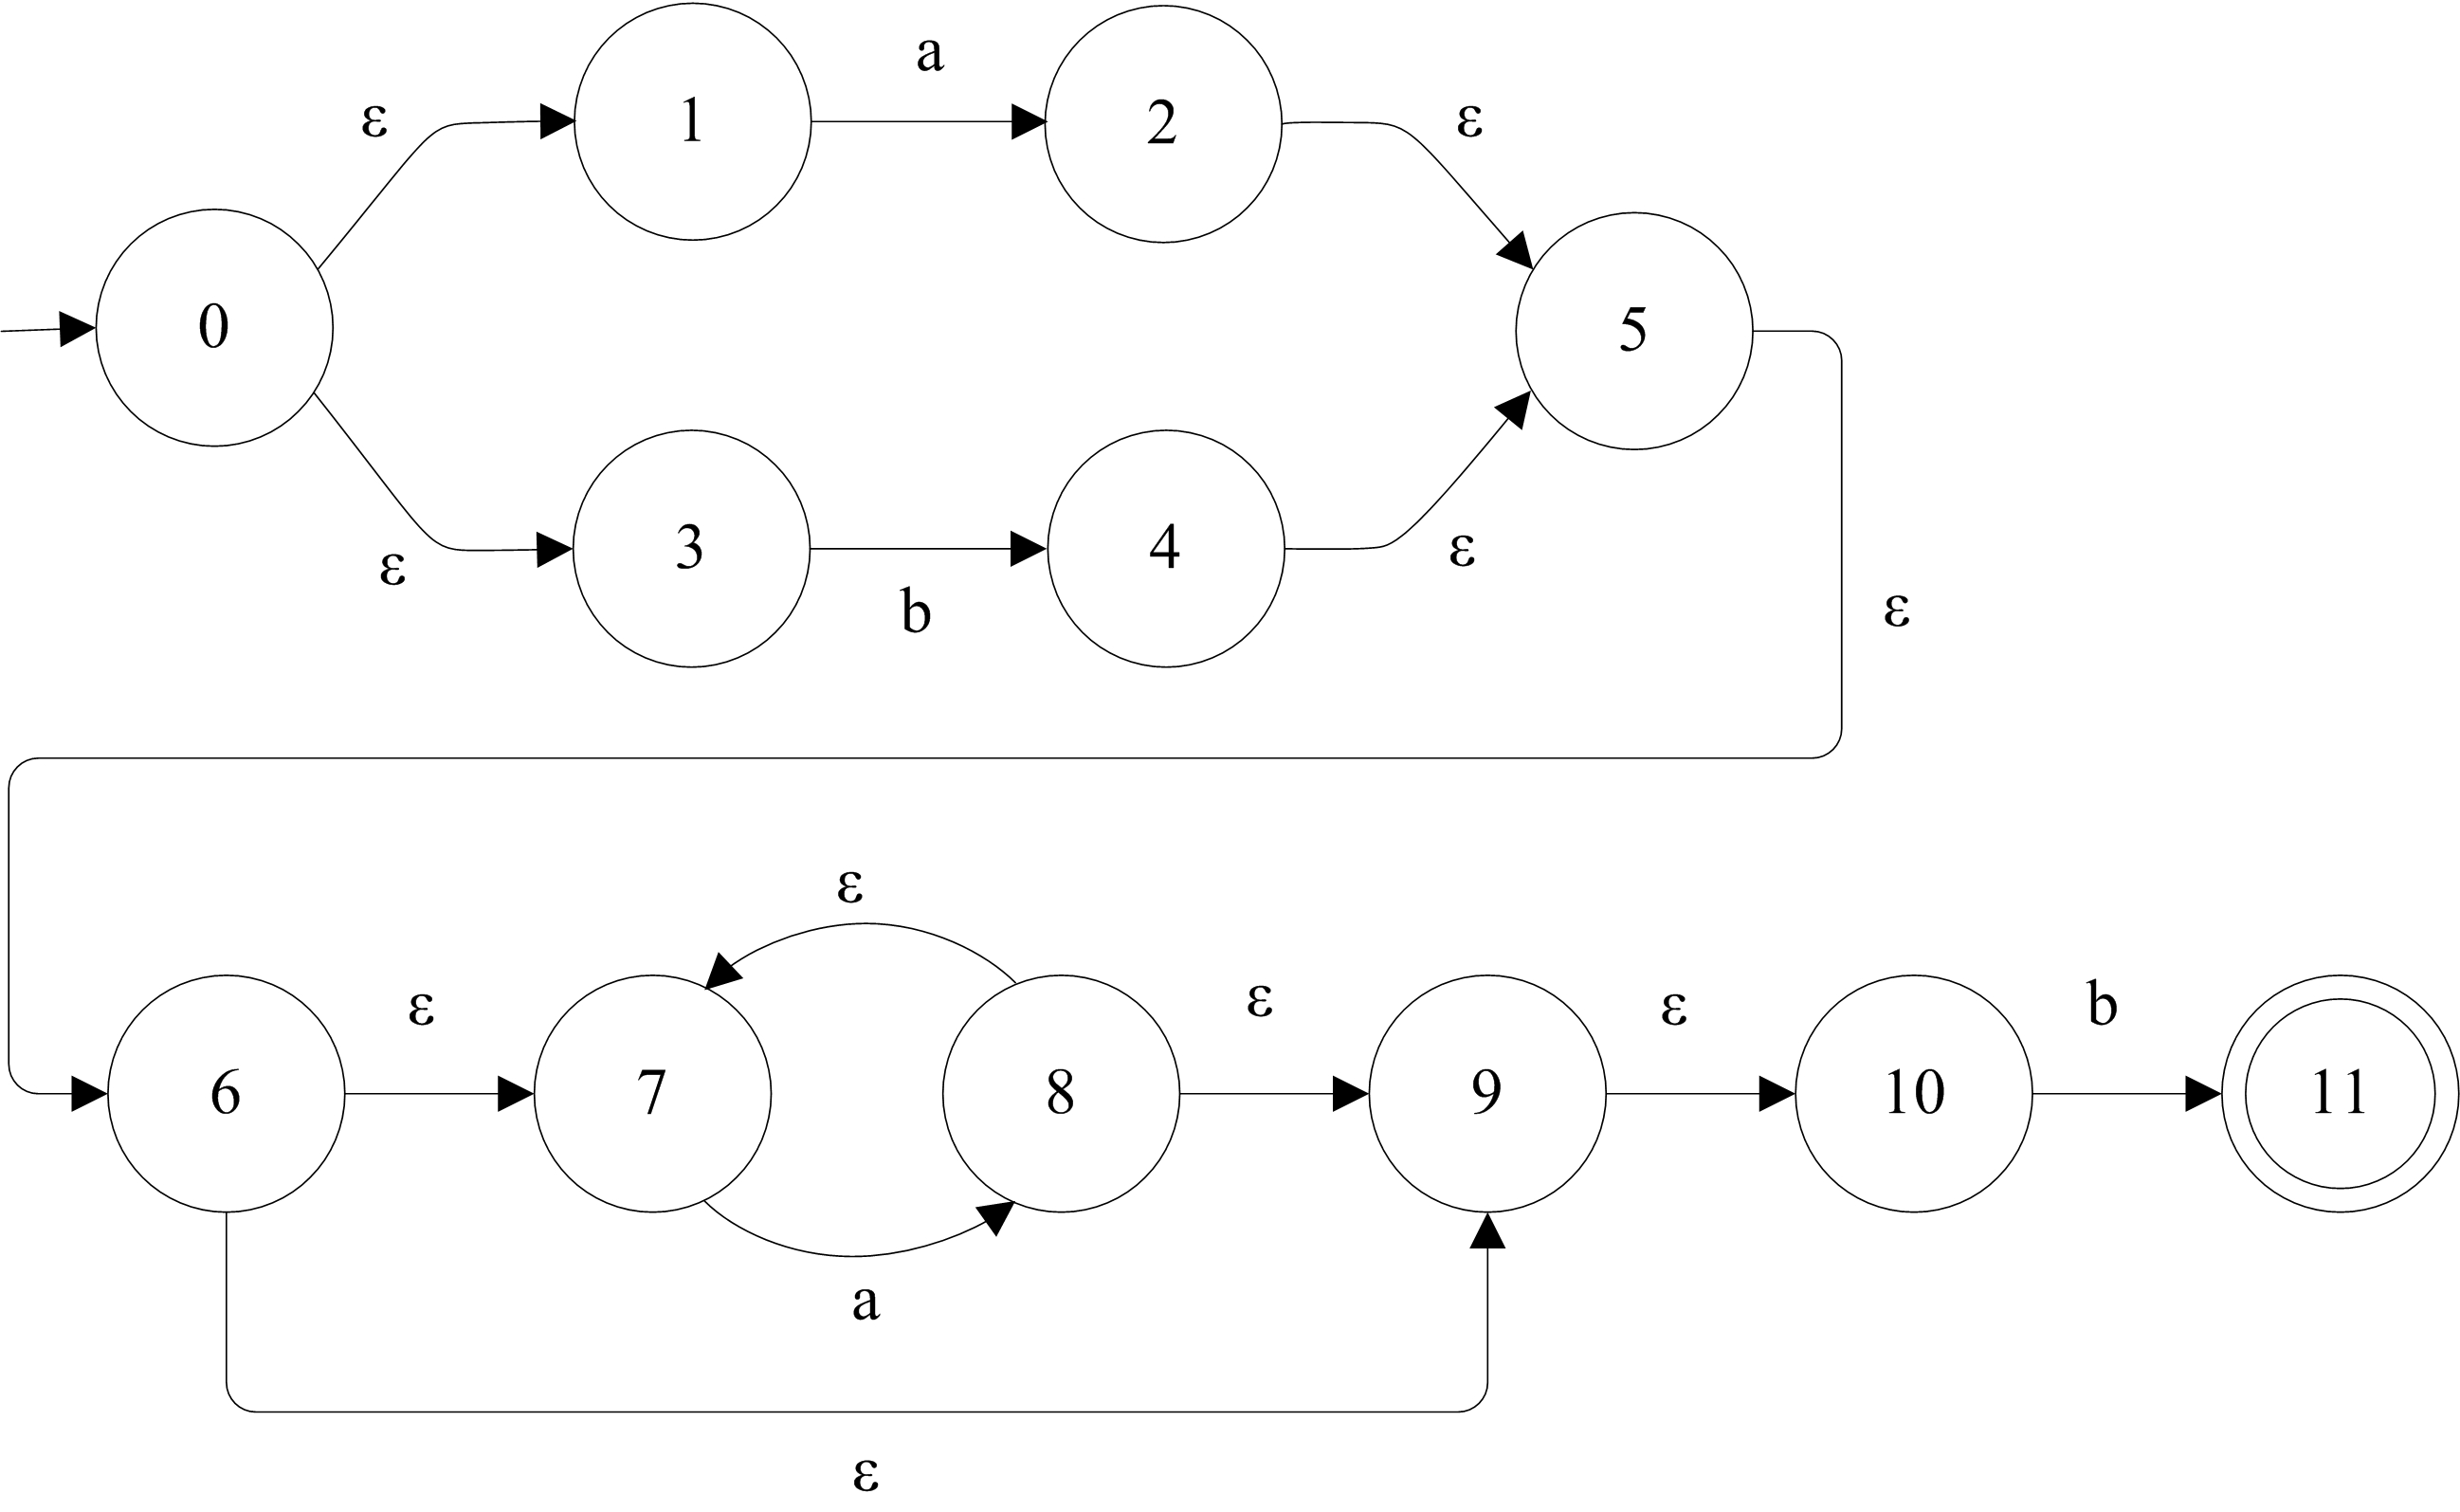
\includegraphics[scale=0.4]{{figures/figure02.15}.jpg}}
\end{center}

\pause
\bigskip

In the corresponding DFA, the start state $s_0 = \epsilon\text{-closure}(0) = \{0, 1, 3\}$

\pause

\begin{align}
& m(s_0, a) = s_1 = \epsilon\text{-closure}(2) = \{2, 5, 6, 7, 9, 10\} \nonumber
\end{align}

\pause

\begin{align}
& m(s_0, b) = s_2 = \epsilon\text{-closure}(4) = \{4, 5, 6, 7, 9, 10\} \nonumber
\end{align}

\pause

\begin{align}
& m(s_1, a) = s_3 = \epsilon\text{-closure}(8) = \{7, 8, 9, 10\} \nonumber
\end{align}

\pause

\begin{align}
& m(s_1, b) = s_4 = \epsilon\text{-closure}(11) = \{11\} \nonumber
\end{align}
\end{frame}

\begin{frame}[fragile]
\pause

\begin{align}
& m(s_2, a) = s_3 \nonumber \\
& m(s_2, b) = s_4 \nonumber
\end{align}

\pause

\begin{align}
& m(s_3, a) = s_3 \nonumber \\
& m(s_3, b) = s_4 \nonumber
\end{align}

\pause
\bigskip

There are no moves at all out of state $s_4$, so we have found all of our transitions and all of our states

\pause
\bigskip

Any state reflecting a final state in the NFA is a final state in the DFA; in our example, only $s_4$ is a final state because it contains (the final) state 11 from the original NFA

\pause
\bigskip

The DFA derived from our NFA for the regular expression $(a|b)a*b$ is shown below
\begin{center}
\visible<6->{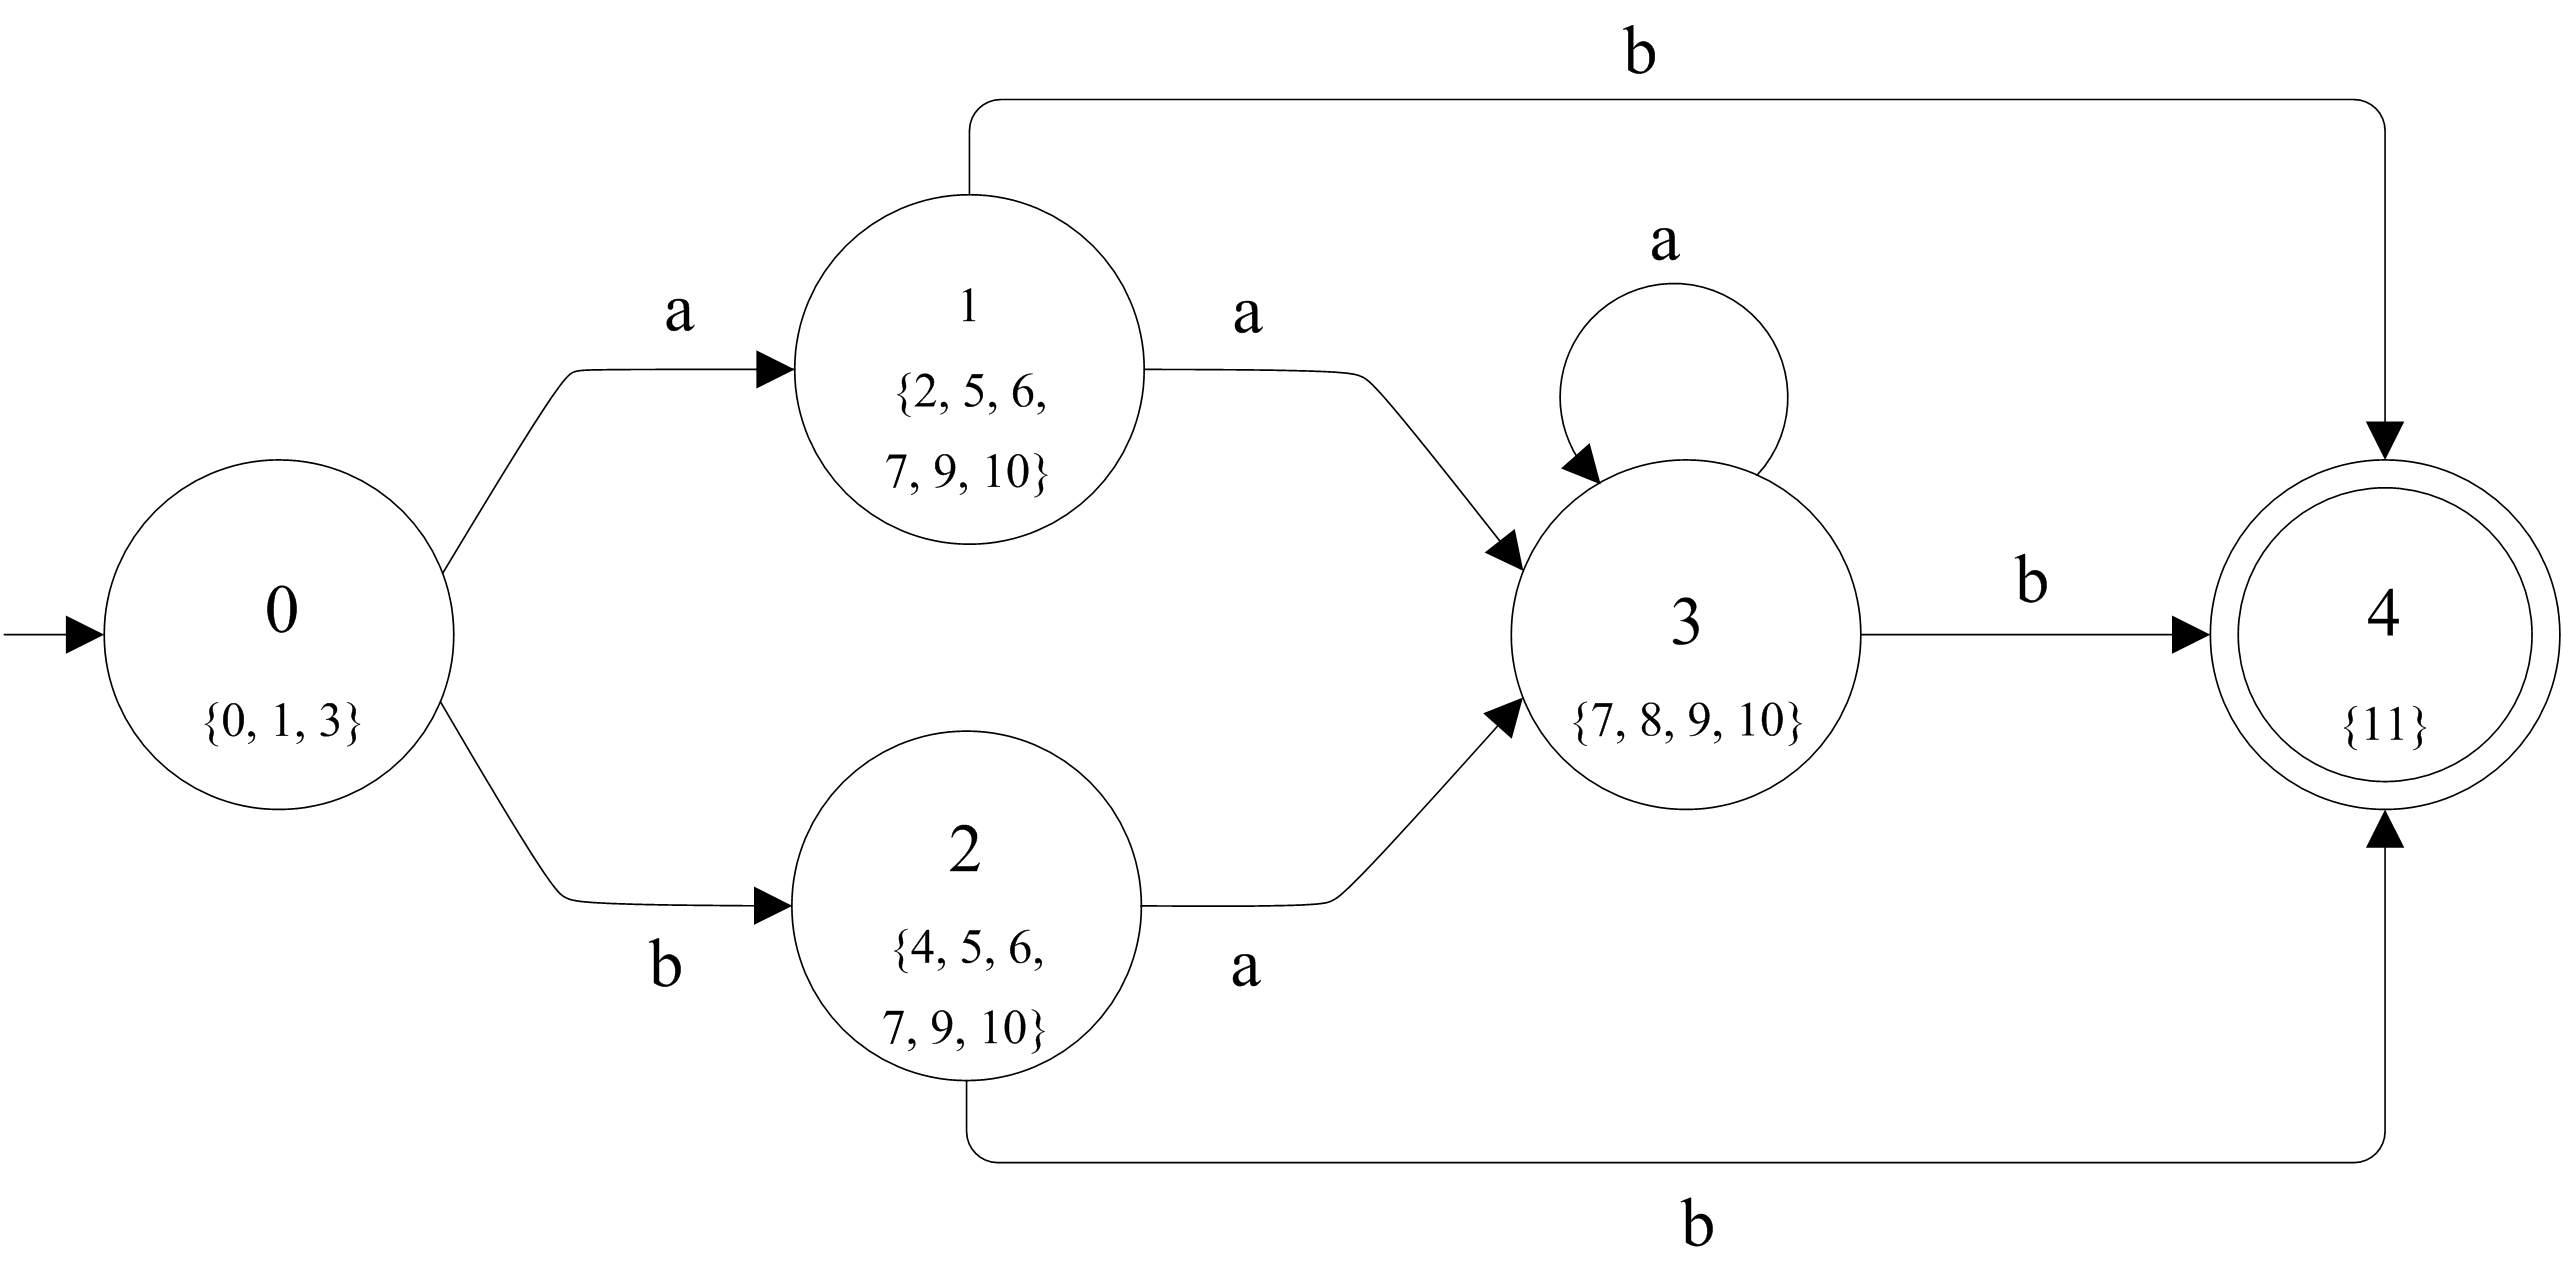
\includegraphics[scale=0.5]{{figures/figure02.16}.jpg}}
\end{center}
\end{frame}

\begin{frame}[fragile]
\pause

\begin{algorithm}[H]
\begin{algorithmic}
\REQUIRE an NFA, $N = (\Sigma, S, s_0, M, F)$
\ENSURE DFA, $D = (\Sigma, S_D, s_{D0}, M_D, F_D)$
\STATE Set $s_{D0} \gets$  $\epsilon$-closure($s_0$)
\STATE Set $S_D$.add($s_{D0}$)
\STATE Moves $M_D$
\STATE Stack $stk$.push($s_{D0}$)
\STATE $i \gets 0$
\WHILE {!$stk$.empty()}
\STATE $t$ $\gets$ $stk$.pop()
\FOR {$a$ in $\Sigma$}
\STATE $s_{Di+1}$ $\gets$ $\epsilon$-closure($m(t, a)$)
\IF {$s_{Di+1} \neq \{\}$}
\IF {$s_{Di+1} \notin S_D$} 
\STATE $S_D$.add($s_{Di+1}$) \COMMENT{We have a new state}
\STATE $stk$.push($s_{Di+1}$)
\STATE $i \gets i + 1$
\STATE $M_D$.add($m_D(t,a) = i$)
\ELSIF {$\exists j, s_j \in S_D \text{ and } s_{Di+1} = s_j$} 
\STATE $M_D$.add($m_D(t, a) = j$) \COMMENT{In the case the state already exists}
\ENDIF
\ENDIF
\ENDFOR
\ENDWHILE
\end{algorithmic}
\caption{NFA to DFA Construction}
\end{algorithm}
\end{frame}

\begin{frame}[fragile]
\pause

\begin{algorithm}[H]
\begin{algorithmic}
\STATE Set $F_D$
\FOR {$s_D$ in $S_D$}
\FOR {$s$ in $s_D$}
\IF {$s \in F$}
\STATE $F_D$.add($s_D$)
\ENDIF
\ENDFOR
\ENDFOR
\RETURN $D = (\Sigma, S_D, s_{D0}, M_D, F_D)$
\end{algorithmic}
\caption{NFA to DFA Construction (contd.)}
\end{algorithm}
\end{frame}

\section{DFA to Minimal DFA}
\begin{frame}[fragile]
\pause

How do we come up with a smaller DFA that recognizes the same language?

\pause
\bigskip

Given an input string in our language, there must be a sequence of moves taking us from the start state to one of the final states

\pause
\bigskip

Given an input string that is not in our language, we must get stuck with no move to take or end up in a non-final state

\pause
\bigskip

We must combine as many states together as we can, so that the states in our new DFA are partitions of the states in the original (perhaps larger) DFA

\pause
\bigskip

A good strategy is to start with just one or two partitions of the states, and then split states when it is necessary to produce the necessary DFA 

\pause
\bigskip

An obvious first partition has two sets: the set of final states and the set of non-final states; the latter could be empty, leaving us with a single partition containing all states
\end{frame}

\begin{frame}[fragile]
\pause

For example, consider the DFA for $(a|b)a*b$, partitioned as follows
\begin{center}
\visible<2->{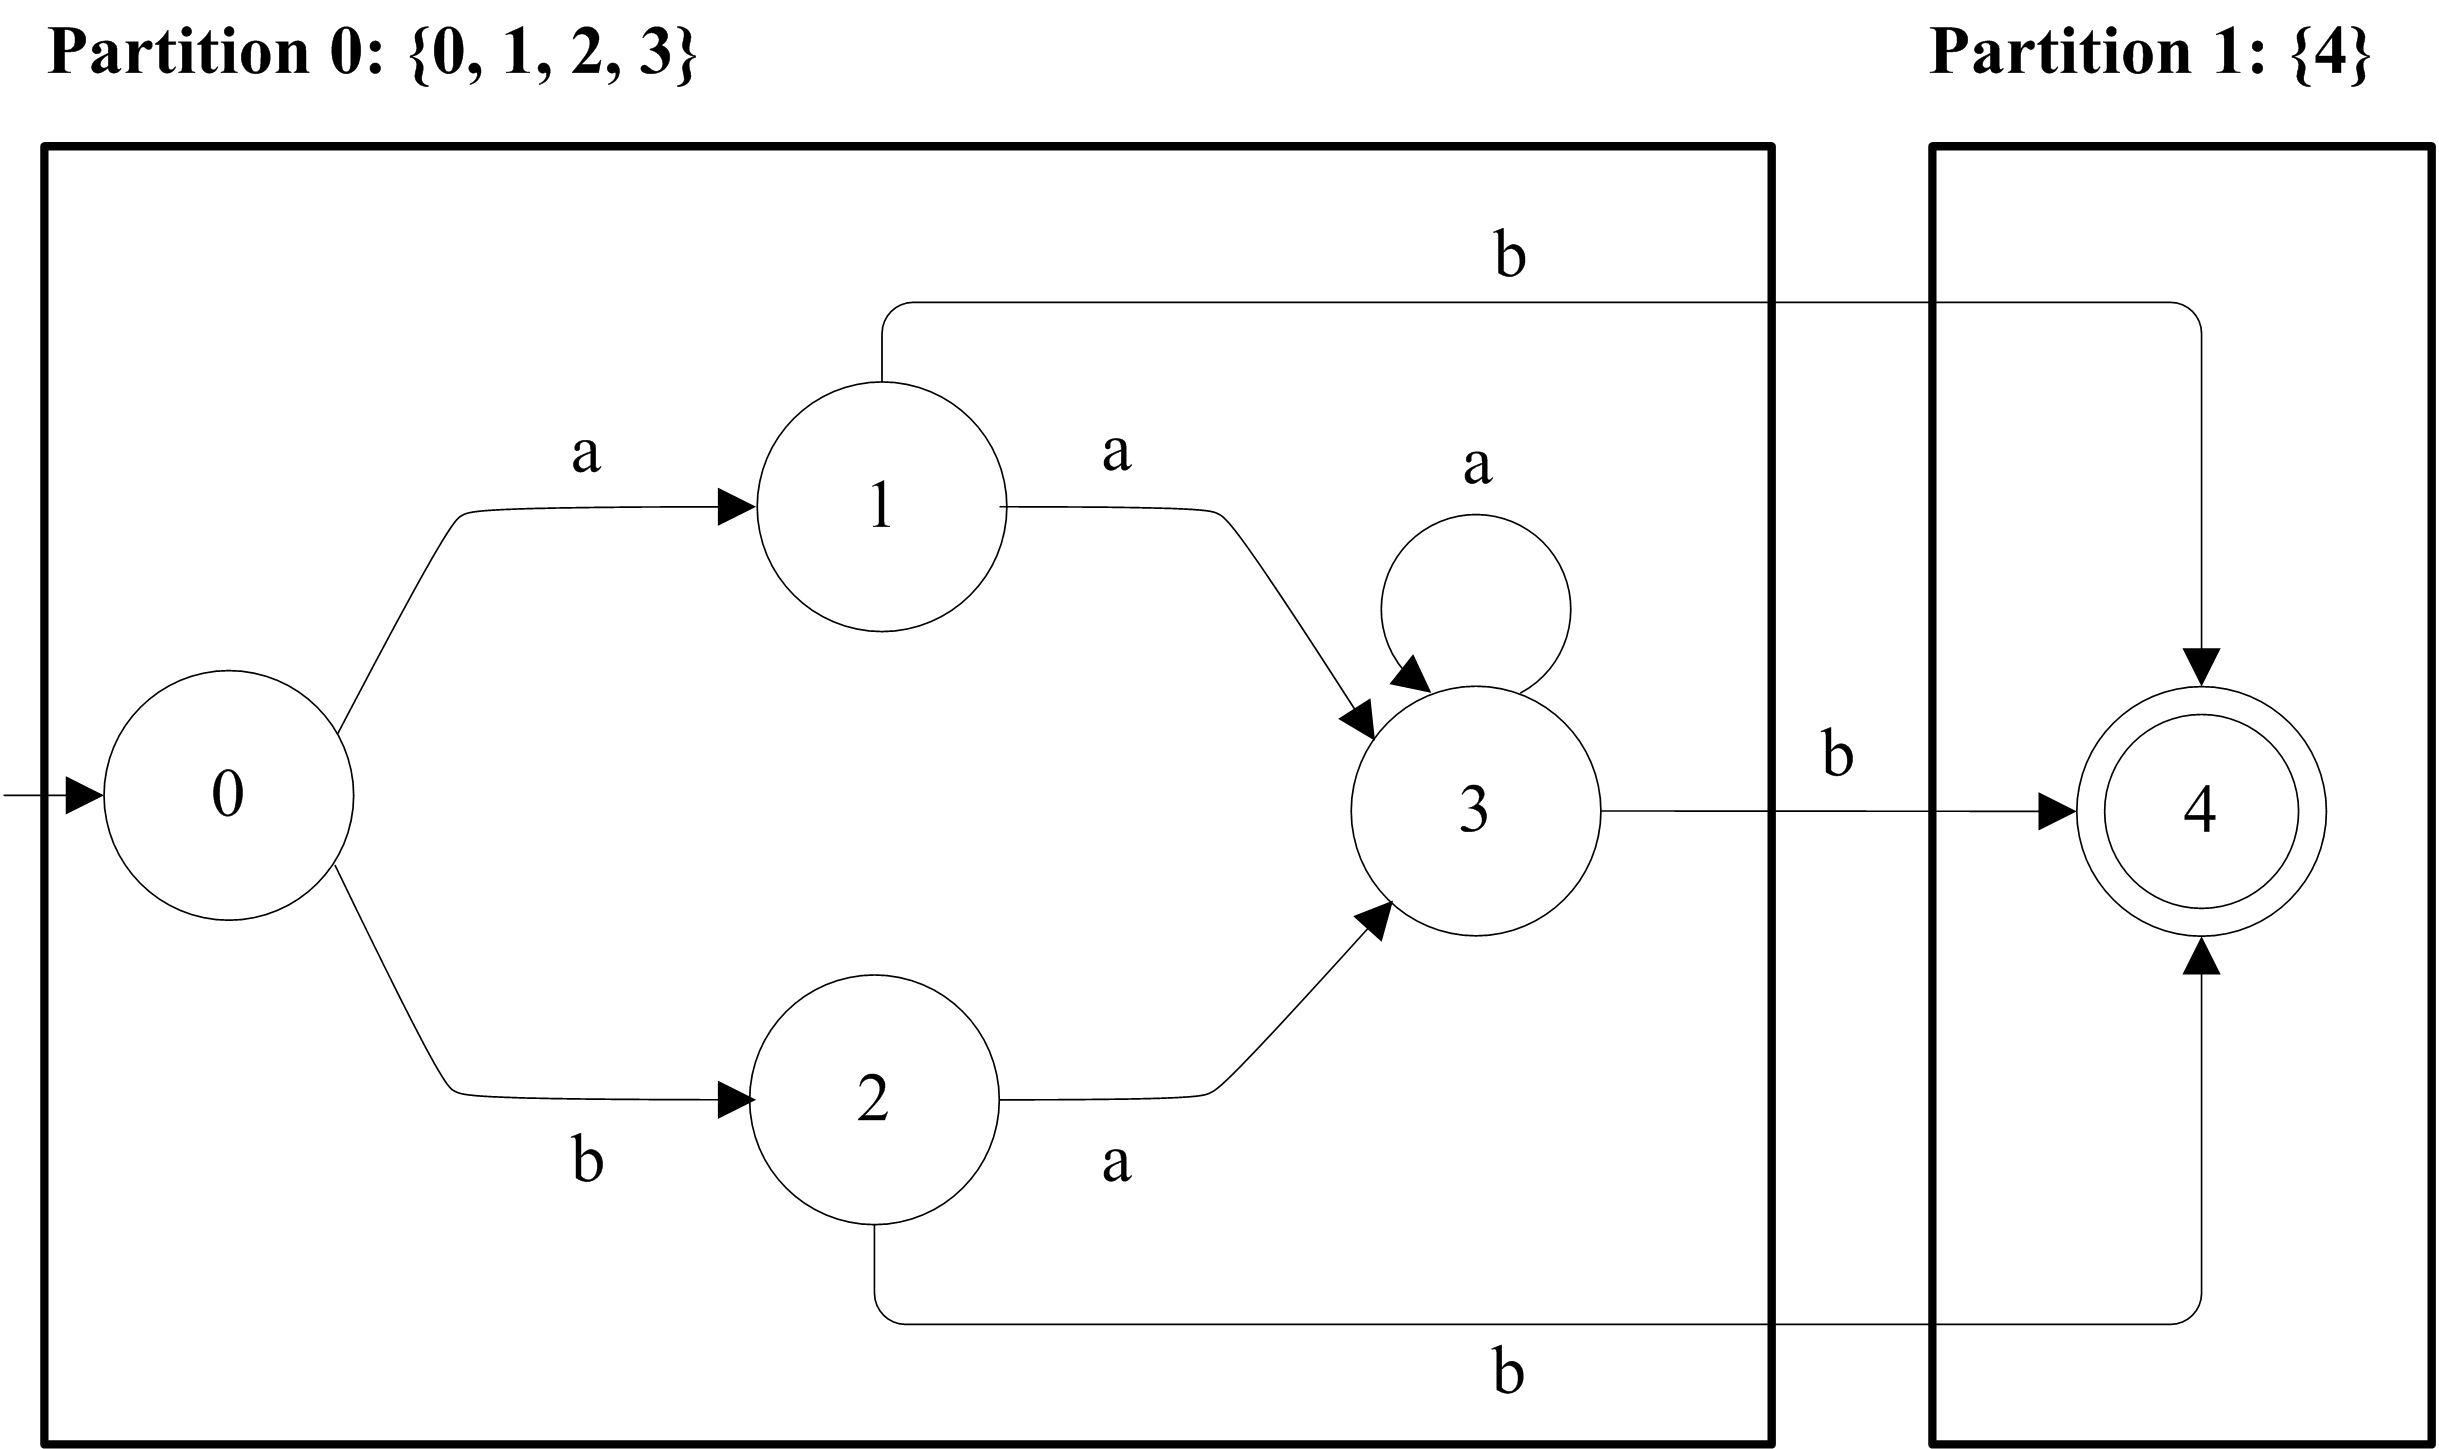
\includegraphics[scale=0.6]{{figures/figure02.17}.jpg}}
\end{center}

\pause
\bigskip

The two states in this new DFA consist of the start state, $\{0, 1, 2, 3\}$ and the final state $\{4\}$ 

\pause
\bigskip

We must make sure that from a particular partition, each input symbol must move us to an identical partition
\end{frame}

\begin{frame}[fragile]
\pause

Beginning in any state in the partition $\{0, 1, 2, 3\}$, an $a$ takes us to one of the states in $\{0, 1, 2, 3\}$
\begin{align}
& m(0, a) = 1 \nonumber \\
& m(1, a) = 3 \nonumber \\
& m(2, a) = 3 \nonumber \\
& m(3, a) = 3 \nonumber
\end{align}

So, our partition $\{0, 1, 2, 3\}$ is fine so far as moves on the symbol $a$ are concerned

\pause
\bigskip

For the symbol $b$,
\begin{align}
& m(0, b) = 2 \nonumber \\
& m(1, b) = 4 \nonumber \\
& m(2, b) = 4 \nonumber \\
& m(3, b) = 4 \nonumber
\end{align}

So we must split the partition $\{0, 1, 2, 3\}$ into two new partitions, $\{0\}$ and $\{1, 2, 3\}$

\pause
\bigskip

If we are in state $s$, and for an input symbol $a$ in our alphabet there is no defined move $m(s, a) = t$, we invent a special dead state $d$, so that we can say $m(s, a) = d$
\end{frame}

\begin{frame}[fragile]
\pause

We are left with a partition into three sets: $\{0\}$, $\{1, 2, 3\}$ and $\{4\}$, as shown below

\begin{center}
\visible<2->{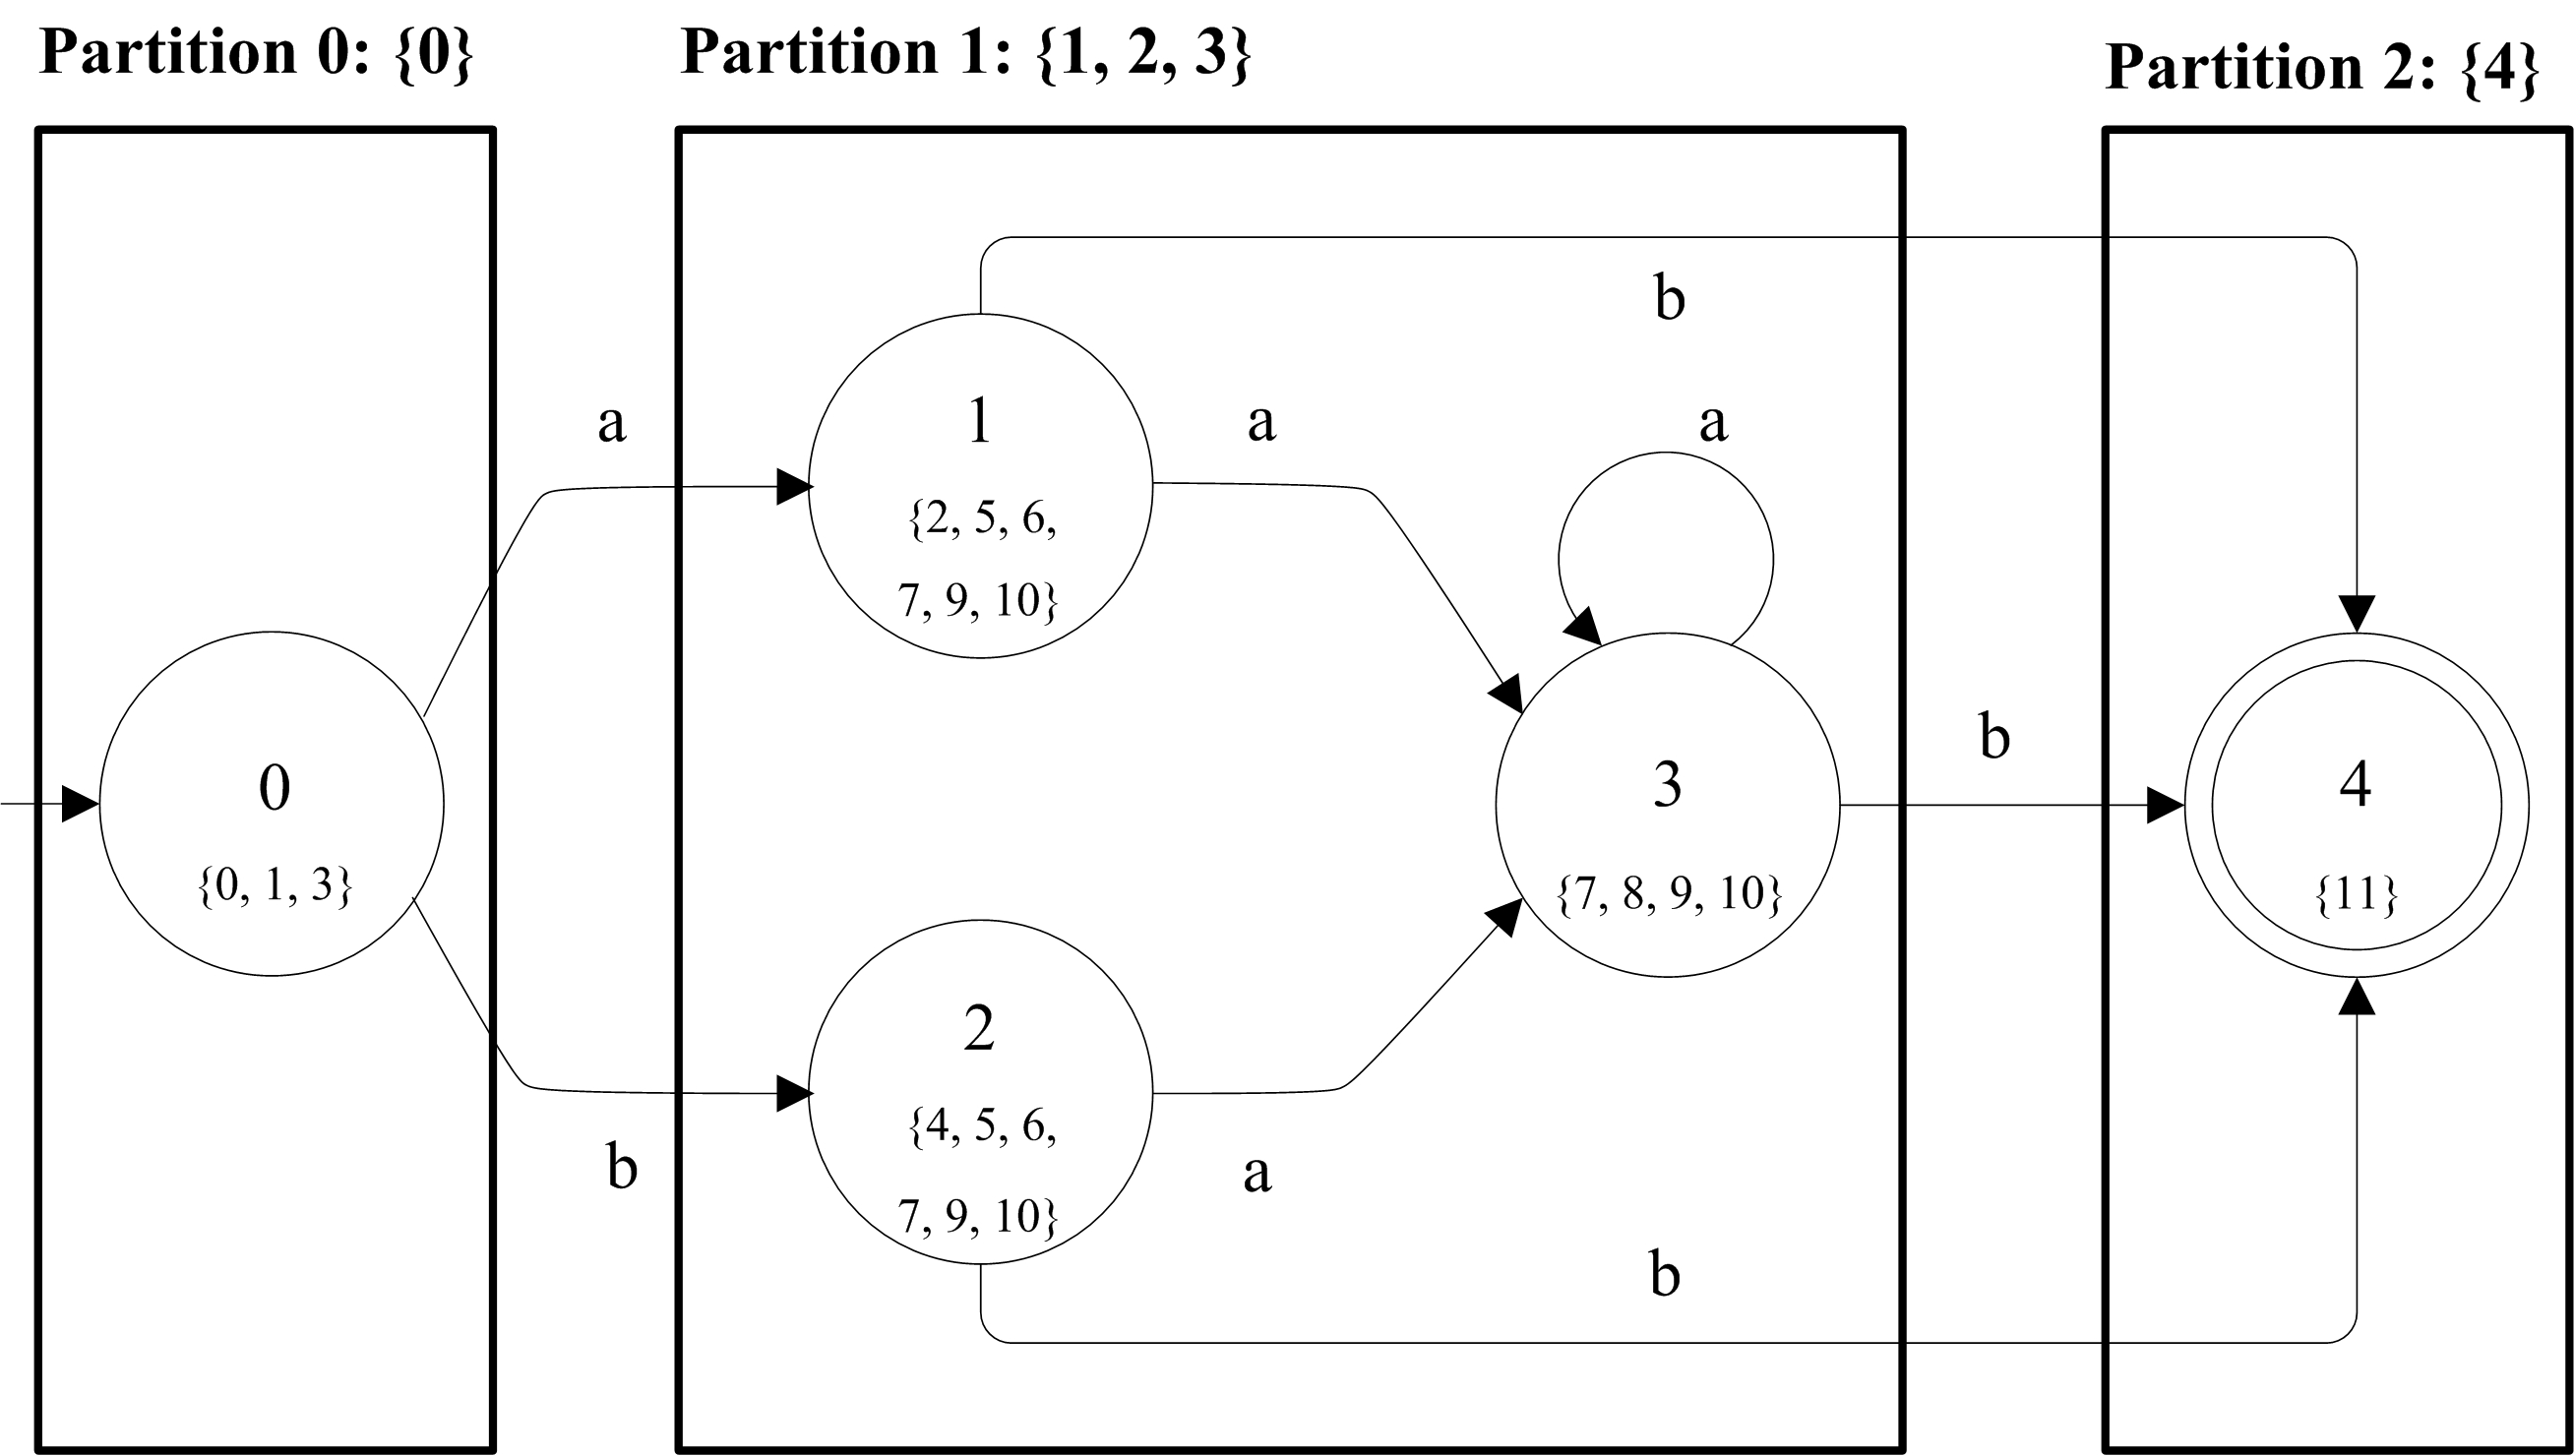
\includegraphics[scale=0.6]{{figures/figure02.18}.jpg}}
\end{center}
\end{frame}

\begin{frame}[fragile]
\pause

We need not worry about $\{0\}$ and $\{4\}$ as they contain just one state and so correspond to (those) states in the original machine

\pause
\bigskip

We consider $\{1, 2, 3\}$ to see if it is necessary to split it
\begin{align}
& m(1,a) = 3\nonumber \\
& m(2,a) = 3 \nonumber \\
& m(3, a) = 3 \nonumber
\end{align}
\begin{align}
& m(1, b) = 4 \nonumber \\
& m(2,b) = 4 \nonumber \\
& m(3, b) = 4 \nonumber
\end{align}

\pause
\bigskip

Thus, there is no further state splitting to be done, and we are left with the following smaller DFA

\begin{center}
\visible<4->{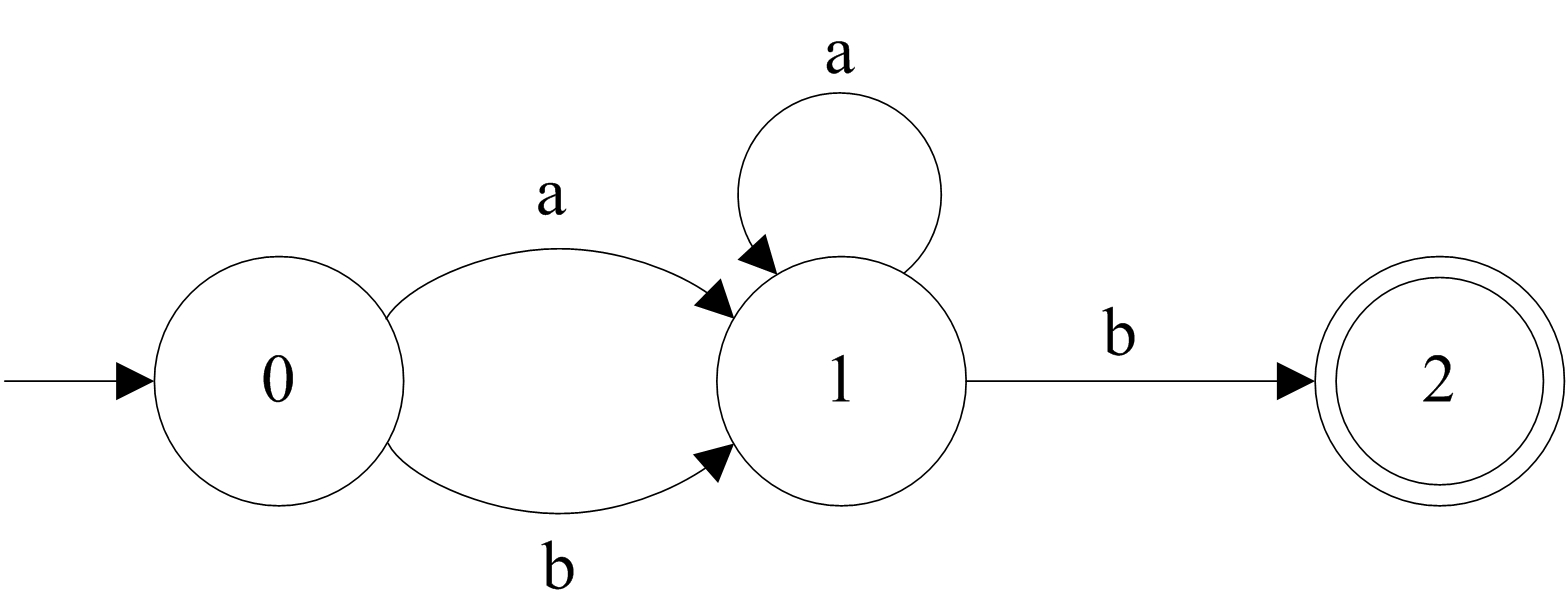
\includegraphics[scale=0.6]{{figures/figure02.19}.jpg}}
\end{center}
\end{frame}

\begin{frame}[fragile]
\pause

\begin{algorithm}[H]
\begin{algorithmic}
\REQUIRE a DFA, $D = (\Sigma, S, s_0, M, F)$
\ENSURE a partition of $S$
\STATE Set $partition \gets \{S - F, F\}$  \COMMENT{start with two sets: the non-final states and the final states} \\
\STATE{} \COMMENT {Splitting the states}
\WHILE {splitting occurs}
\FOR {Set $set$  in $partition$}
\IF {$set$.size() $>$ 1}
\FOR {Symbol $a$ in $\Sigma$}
\STATE{} \COMMENT{Determine if  moves from this `state' force a split}
\STATE State $s \gets$ a state chosen from $set$
\STATE $targetSet \gets$ the set in the partition containing $m(s, a)$
\STATE Set $set1 \gets \{\text{states } s \text{ from set } S, \text{ such that } m(s, a) \in targetSet\}$
\STATE Set $set2 \gets \{\text{states } s \text{ from set } S, \text{ such that } m(s, a) \notin targetSet\}$
\IF {$set2 \neq \{\}$}
\STATE{} \COMMENT{Yes, split the states.}
\STATE{replace $set$ in $partition$ by $set1$ and $set2$ and break out of the for-loop to continue with the next set in the partition}
\ENDIF
\ENDFOR
\ENDIF
\ENDFOR
\ENDWHILE
\end{algorithmic}
\caption{Minimizing a DFA}
\end{algorithm}
\end{frame}

\begin{frame}[fragile]
\pause

Let us run through another example, starting from a regular expression, producing an NFA, then a DFA, and finally a minimal DFA

\pause
\bigskip

Consider the regular expression $(a|b)*baa$ having the following syntactic structure

\begin{center}
\visible<3->{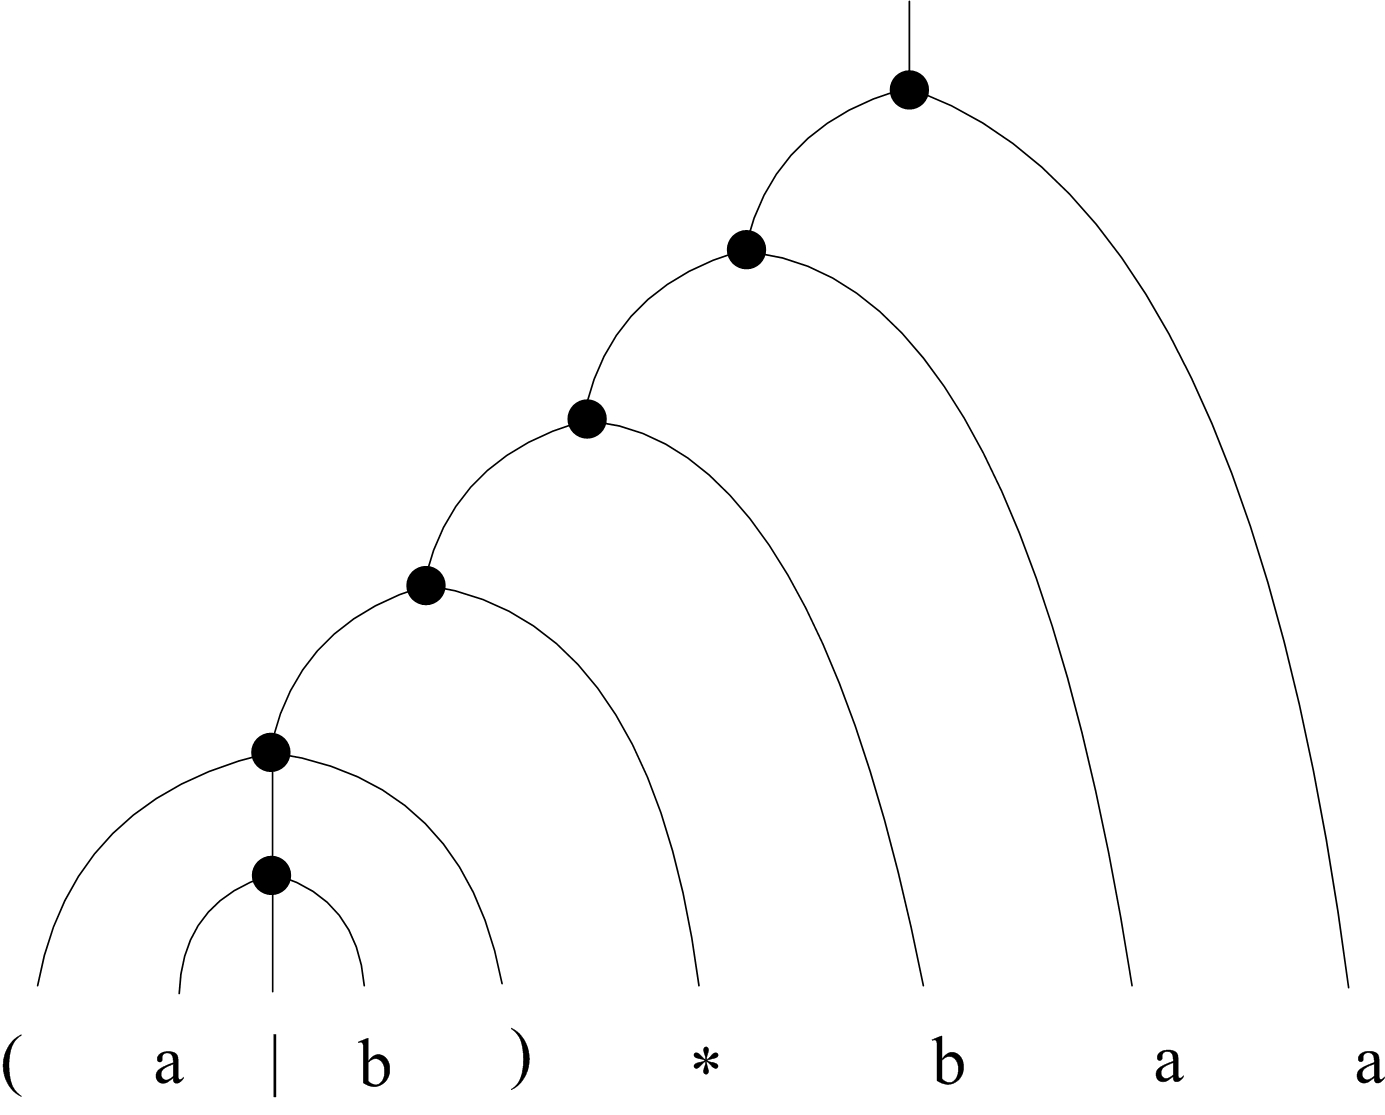
\includegraphics[scale=0.6]{{figures/figure02.20}.jpg}}
\end{center}
\end{frame}

\begin{frame}[fragile]
\pause

We apply the Thompson's construction procedure to produce the NFA shown below
\begin{center}
\visible<2->{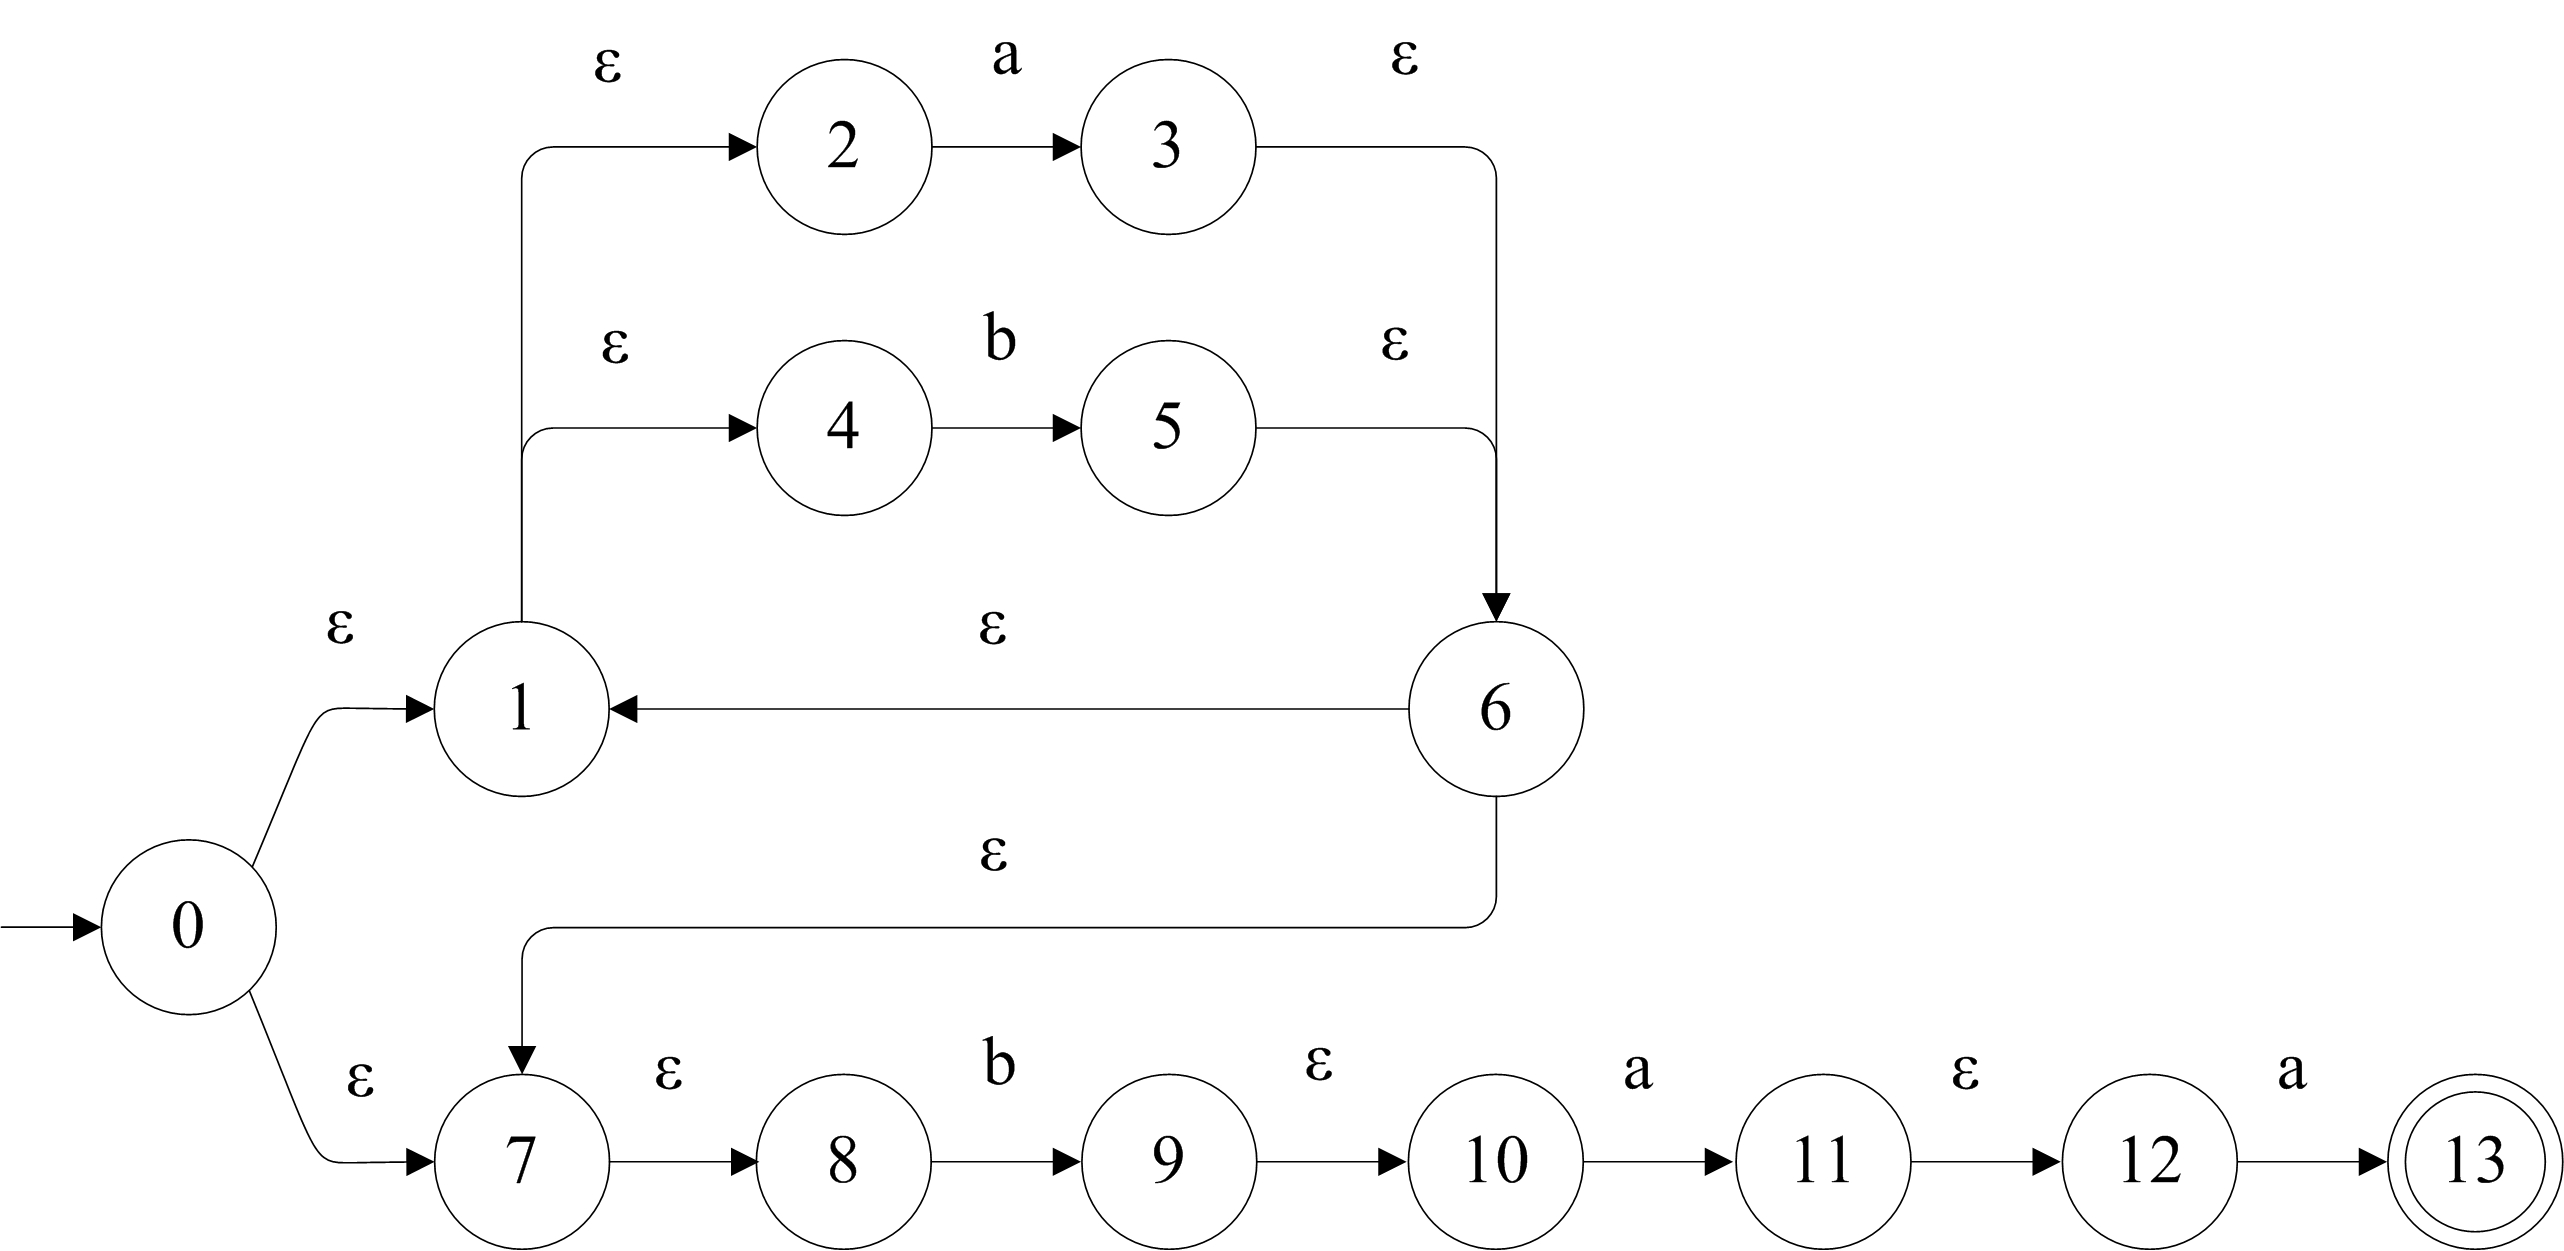
\includegraphics[scale=0.6]{{figures/figure02.21}.jpg}}
\end{center}
\end{frame}

\begin{frame}[fragile]
\pause

Using the powerset construction method, we derive a DFA having the following states
\begin{align}
& s_0 = \{0, 1, 2, 4, 7, 8\} \nonumber \\
& m(s_0, a) : \{1, 2, 3, 4, 6, 7, 8\} = s_1 \nonumber \\
& m(s_0, b) : \{1, 2, 4, 5, 6,  7, 8, 9, 10\} = s_2 \nonumber \\
& m(s_1, a) : \{1, 2, 3, 4, 6, 7, 8\} = s_1 \nonumber \\
& m(s_1, b) : \{1, 2, 4, 5, 6, 7, 8, 9, 10\} = s_2 \nonumber \\
& m(s_2, a) : \{1, 2, 3, 4, 6, 7, 8, 11, 12\} = s_3 \nonumber \\
& m(s_2, b) : \{1, 2, 4, 5, 6, 7, 8, 9, 10\} = s_2 \nonumber \\
& m(s_3, a) : \{1, 2, 3, 4, 6, 7, 8, 13\} = s_4 \nonumber \\
& m(s_3, b) : \{1, 2, 4, 5, 6, 7, 8, 9, 10\} = s_2 \nonumber \\
& m(s_4, a) : \{1, 2, 3, 4, 6, 7, 8\} = s_1 \nonumber \\
& m(s_4, b) : \{1, 2, 4, 5, 6, 7, 8, 9, 10\} = s_2 \nonumber
\end{align}
\end{frame}

\begin{frame}[fragile]
\pause

The DFA itself is shown below
\begin{center}
\visible<2->{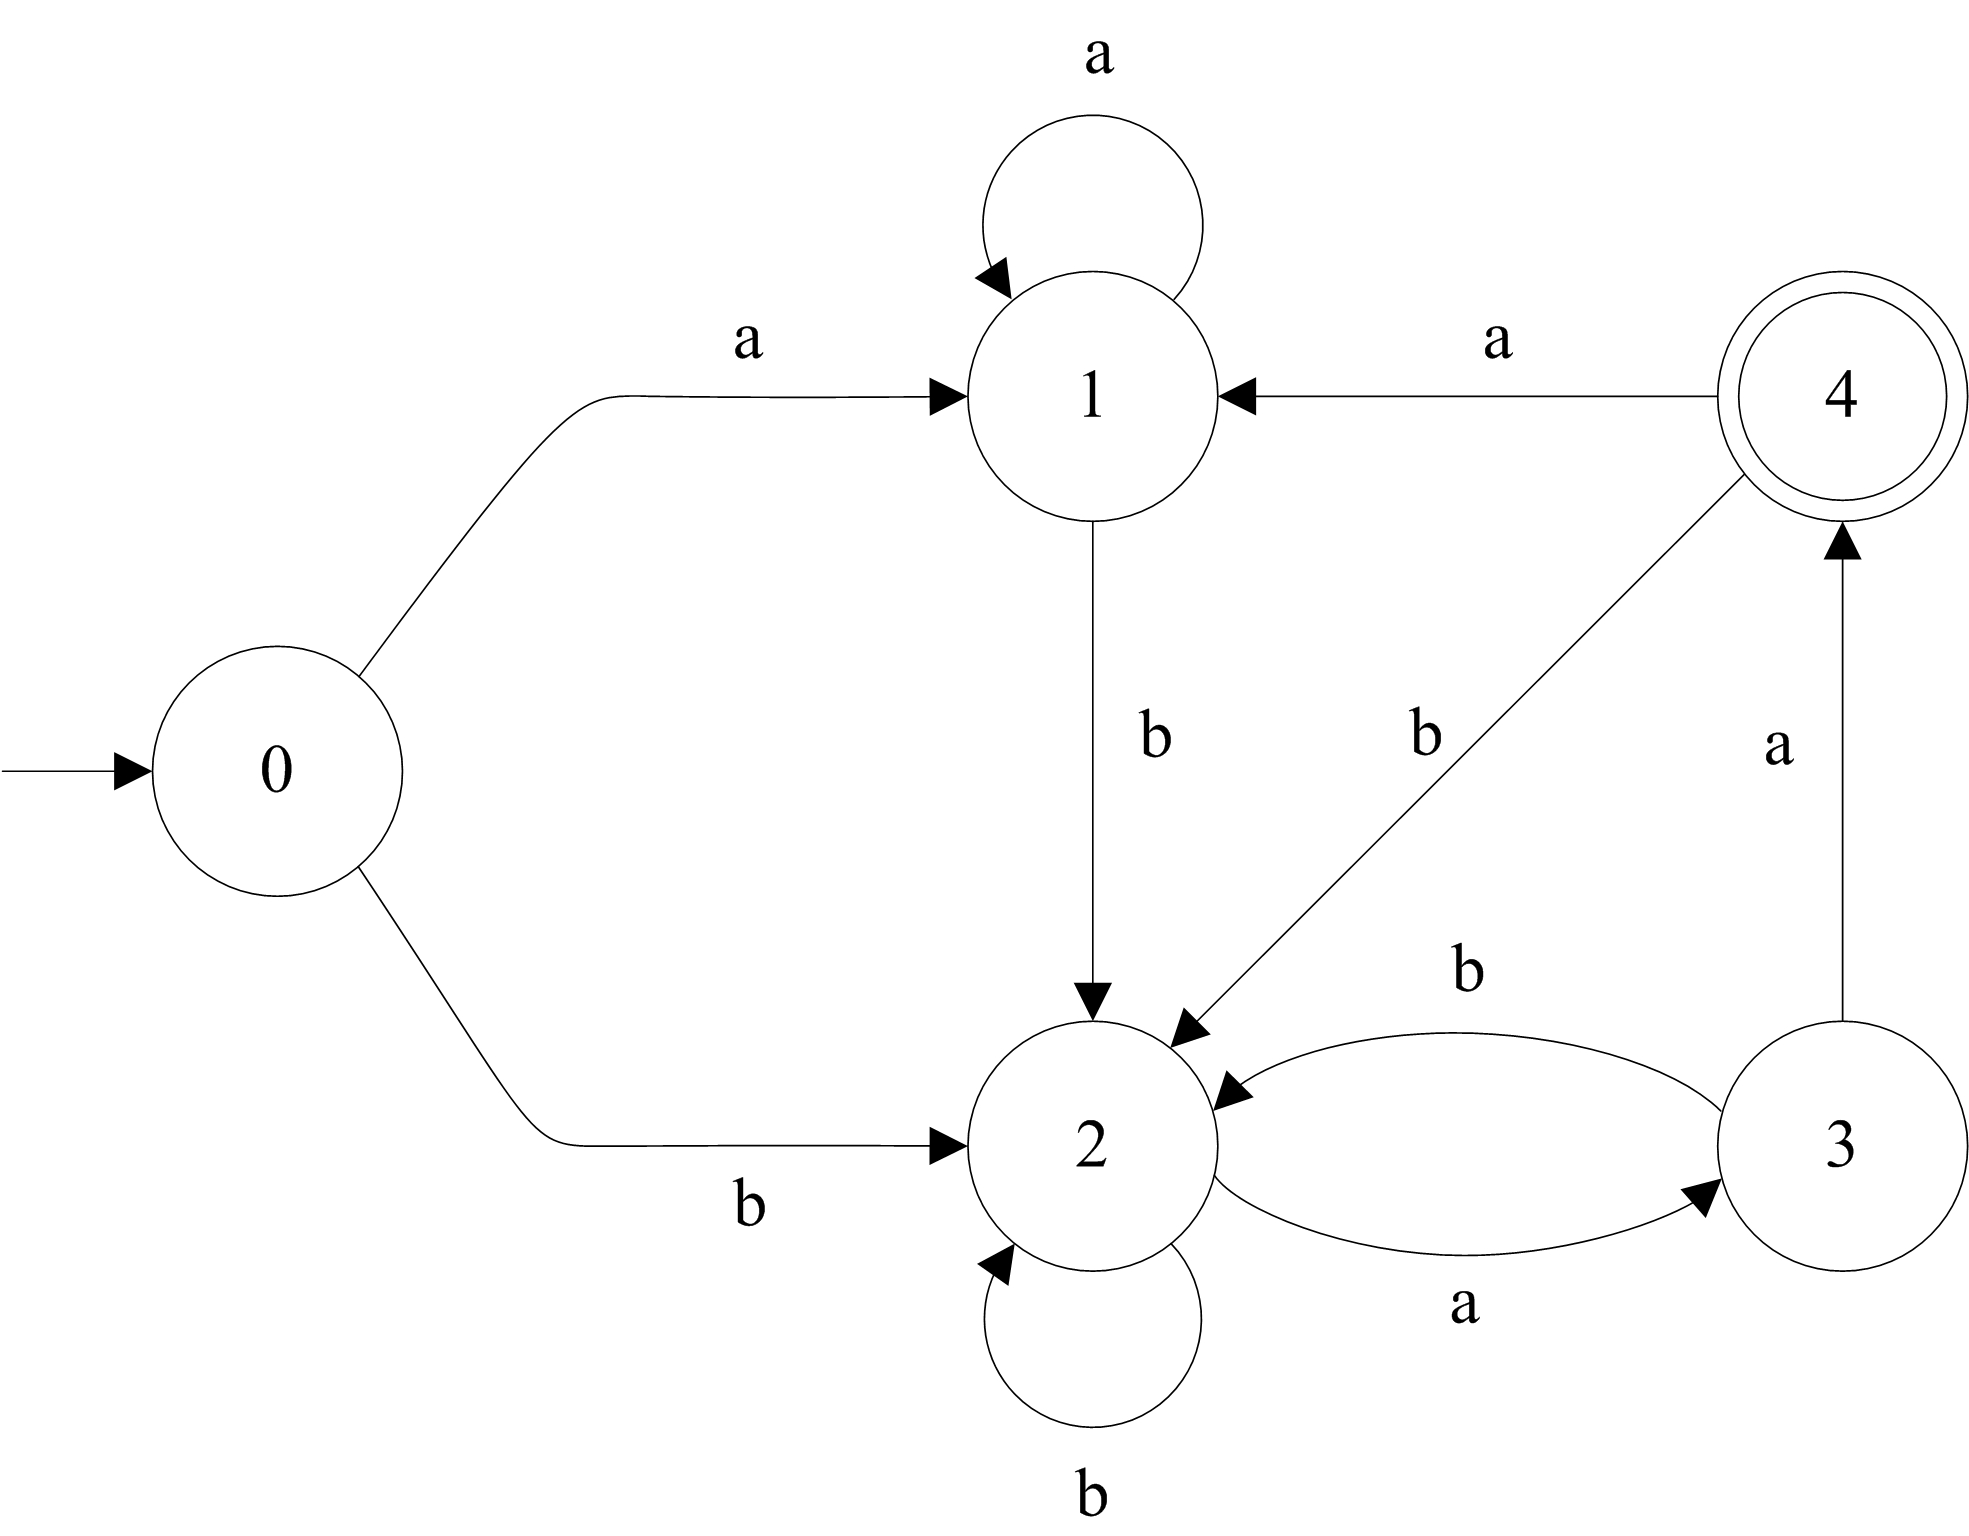
\includegraphics[scale=0.6]{{figures/figure02.22}.jpg}}
\end{center}
\end{frame}

\begin{frame}[fragile]
\pause

Finally, we use partitioning to produce the minimal DFA shown below
\begin{center}
\visible<2->{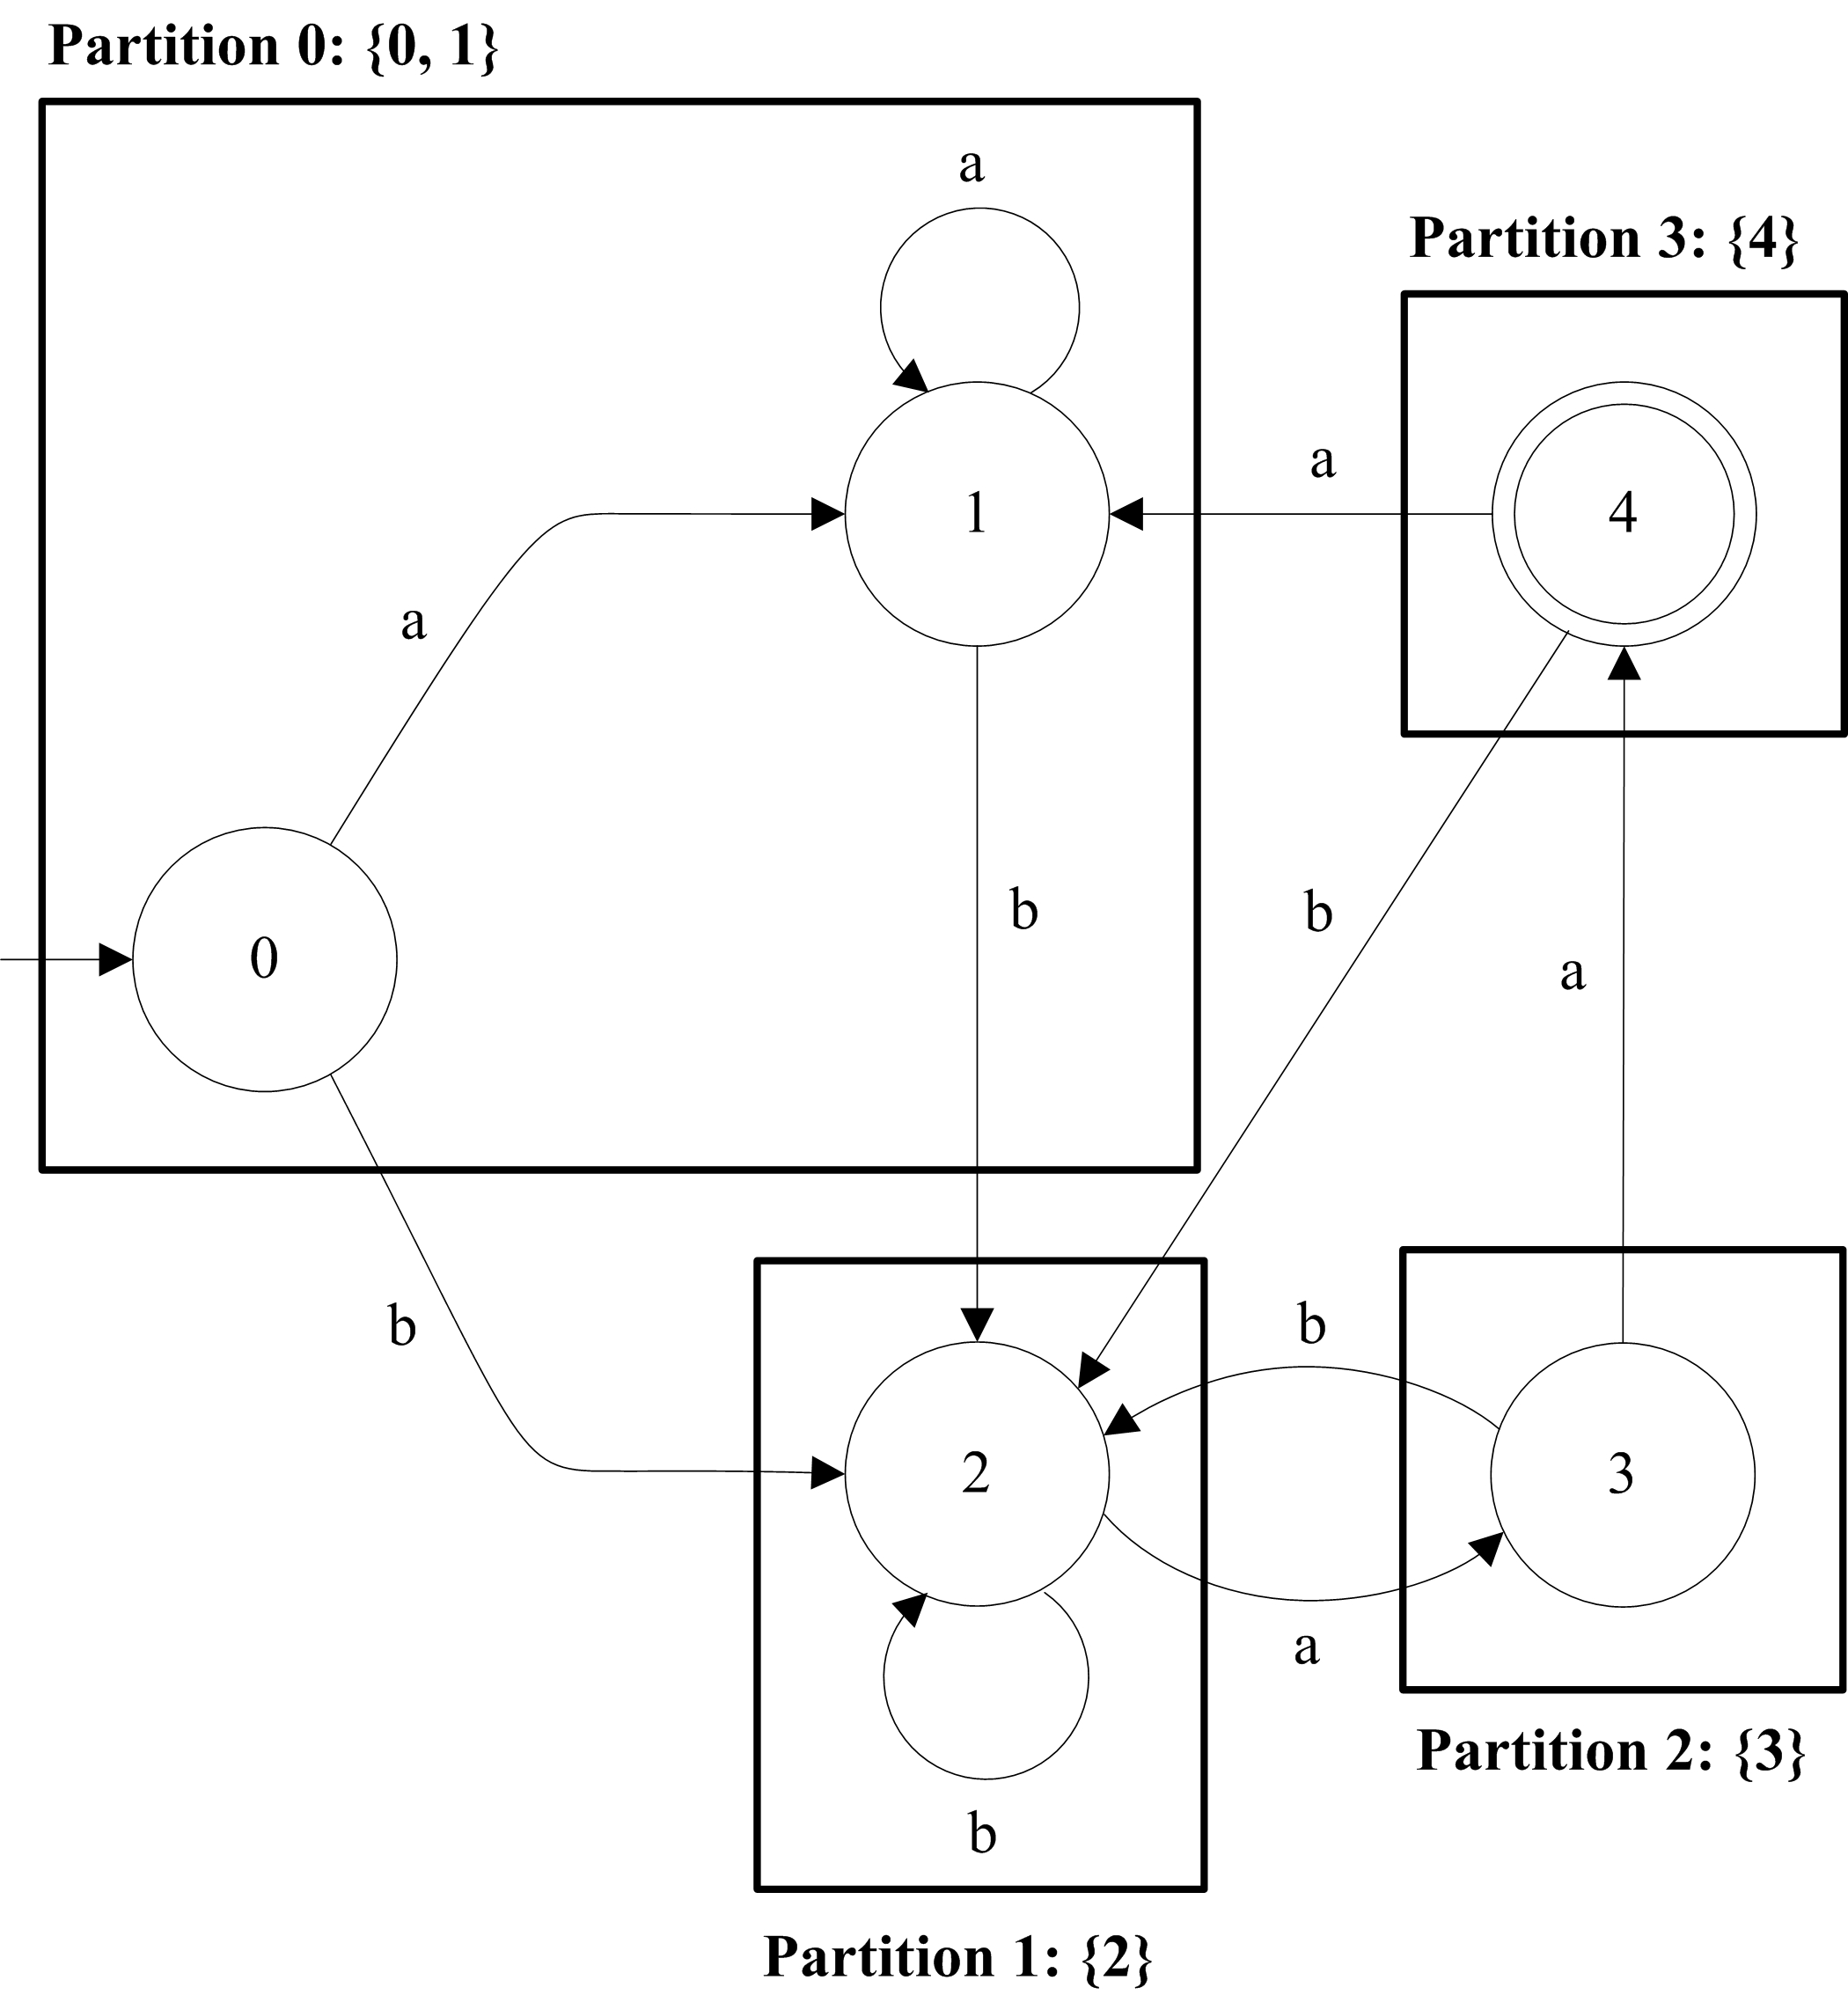
\includegraphics[scale=0.6]{{figures/figure02.23}.jpg}}
\end{center}
\end{frame}

\begin{frame}[fragile]
\pause

We re-number the states to produce the equivalent DFA shown below
\begin{center}
\visible<2->{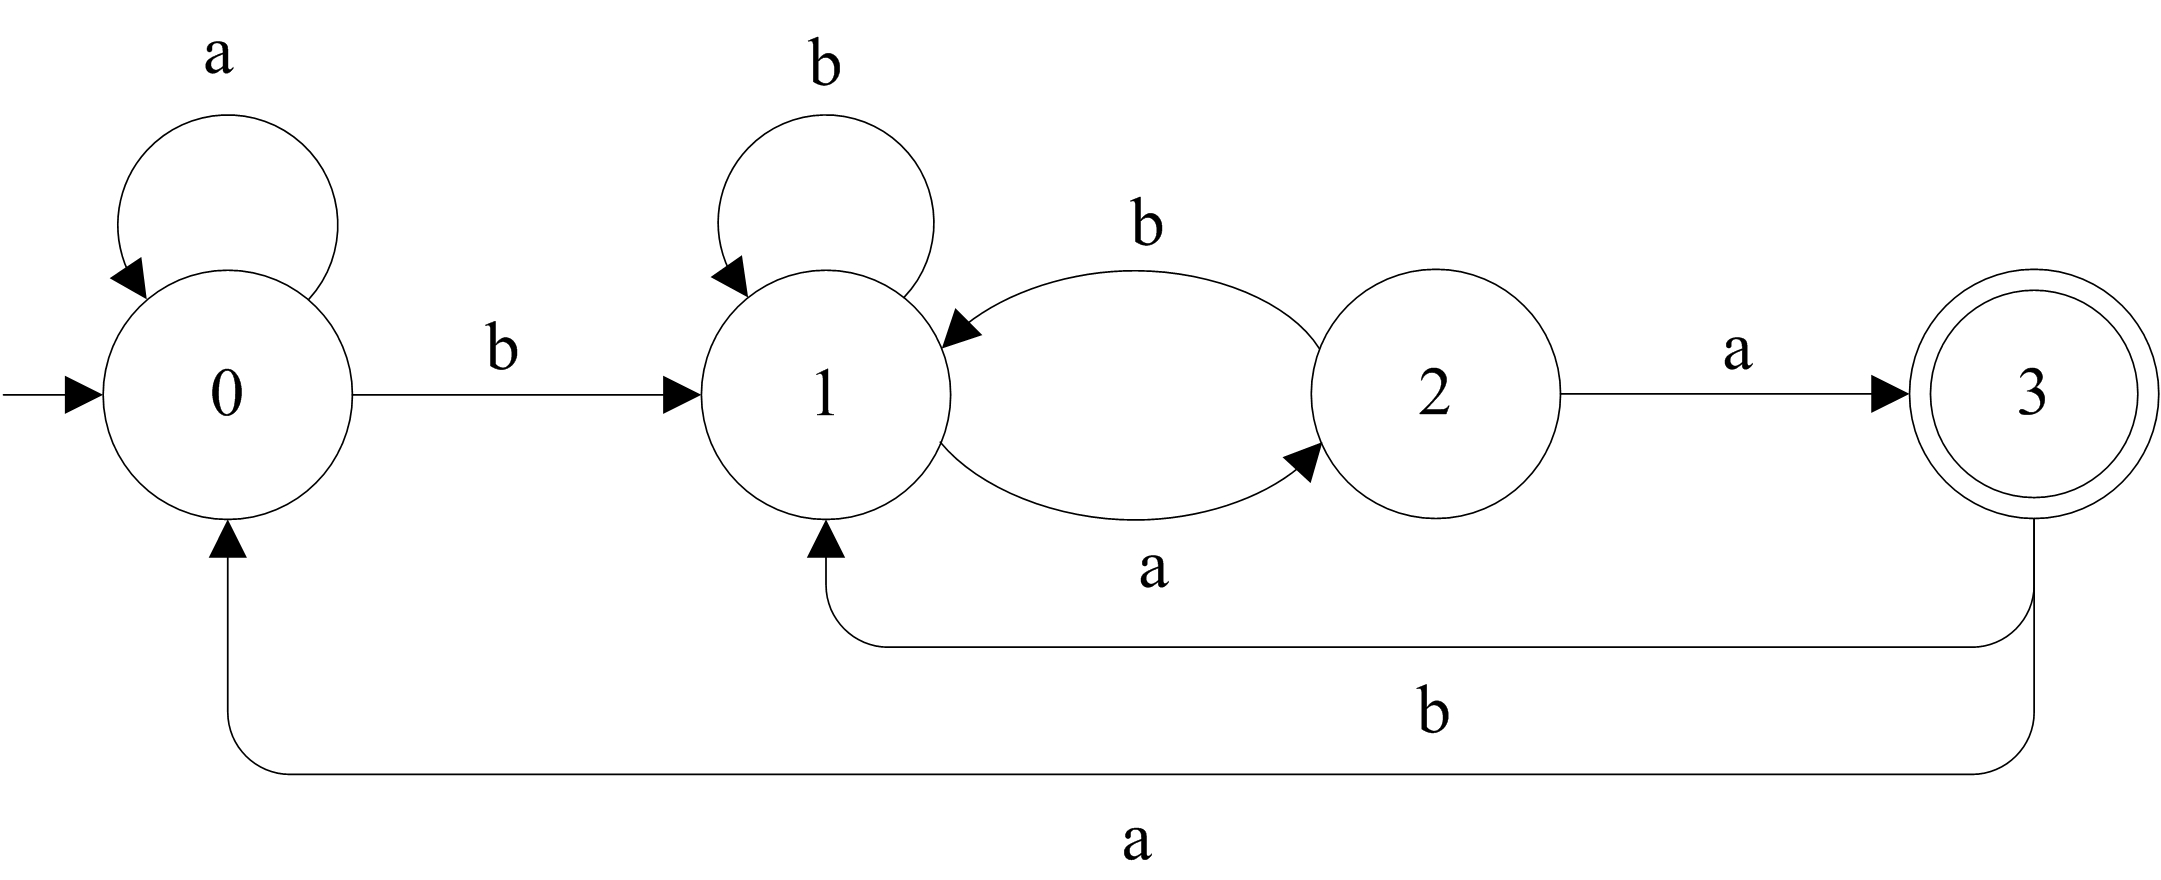
\includegraphics[scale=0.6]{{figures/figure02.24}.jpg}}
\end{center}
\end{frame}

\section{JavaCC: a Tool for Generating Scanners}
\begin{frame}[fragile]
\pause

JavaCC (the CC stands for compiler-compiler) is a tool for generating lexical analyzers from regular expressions and parsers from context-free grammars

\pause
\bigskip

A lexical grammar specification consists a set of regular expressions and a set of lexical states; from any particular state, only certain regular expressions may be matched in scanning the input

\pause
\bigskip

There is a standard \lstinline{DEFAULT} state, in which scanning generally begins; one may specify additional states as required

\pause
\bigskip

Scanning a token proceeds by considering all regular expressions in the current state and choosing the one which consumes the greatest number of input characters

\pause
\bigskip

After a match, one can specify a state in which the scanner should go into; otherwise the scanner stays in the current state

\pause
\bigskip

There are four kinds of regular expressions, determining what happens when the regular expression has been matched
\begin{enumerate}
\item \lstinline{SKIP}: throws away the matched string
\item \lstinline{MORE}: continues to the next state, taking the matched string along
\item \lstinline{TOKEN}: creates a token from the matched string and returns it to the parser (or any caller)
\item \lstinline{SPECIAL_TOKEN}: creates a special token that does not participate in the parsing
\end{enumerate}
\end{frame}

\begin{frame}[fragile]
\pause

For example, a \lstinline{SKIP} can be used for ignoring white space
\begin{lstlisting}[language={}]
SKIP: {" "|"\t"|"\n"|"\r"|"\f"}
\end{lstlisting}

\pause
\bigskip

We can deal with single-line comments with the following regular expressions

\begin{lstlisting}
MORE: { "//": IN_SINGLE_LINE_COMMENT }
<IN_SINGLE_LINE_COMMENT>
SPECIAL_TOKEN: { <SINGLE_LINE_COMMENT: "\n"|"\r"|"\r\n" > : DEFAULT }
<IN_SINGLE_LINE_COMMENT>
MORE: { < ~[] > }
\end{lstlisting}

\pause
\bigskip

An alternative regular expression dealing with single-line comments

\begin{lstlisting}
SPECIAL_TOKEN: {
  <SINGLE_LINE_COMMENT: "//" (~["\n","\r"])* ("\n"|"\r"|"\r\n")>
}
\end{lstlisting}

\pause
\bigskip

Reserved words and symbols are specified by simply spelling them out; for example

\begin{lstlisting}
TOKEN: {
  < ABSTRACT: "abstract" >
| < BOOLEAN: "boolean" >
...

| < COMMA: "," >
| < DOT: "." >
}
\end{lstlisting}
\end{frame}

\begin{frame}[fragile]
\pause

A token for scanning identifiers

\begin{lstlisting}
TOKEN: {
  < IDENTIFIER: (<LETTER>|"_"|"$") (<LETTER>|<DIGIT>|"_"|"$")* >
| < #LETTER: ["a"-"z","A"-"Z"] >
| < #DIGIT: ["0"-"9"] >
}
\end{lstlisting}

\pause
\bigskip

A token for scanning literals

\begin{lstlisting}
TOKEN: {
  < INT_LITERAL: ("0" | <NON_ZERO_DIGIT> (<DIGIT>)*) >
| < #NON_ZERO_DIGIT: ["1"-"9"] >
| < CHAR_LITERAL: "'" (<ESC> | ~["'","\\","\n","\r"]) "'" >
| < STRING_LITERAL: "\"" (<ESC> | ~["\"","\\","\n","\r"])* "\"" >
| < #ESC: "\\" ["n","t","b","r","f","\\","'","\""] >
}
\end{lstlisting}

\pause
\bigskip

JavaCC takes a specification of the lexical syntax and produces several Java files, one of which is  \lstinline{TokenManager.java}, a program that implements a state machine; this is our scanner

\pause
\bigskip

The lexical specification for \jmm is contained in \lstinline{$j/j--/src/jminusminus/j--.jj}
\end{frame}
\end{document}
